\documentclass[format=acmsmall, review=false, screen=true]{acmart}
\usepackage{booktabs} % For formal tables
\usepackage{makecell}
\usepackage{lipsum}
\usepackage[utf8]{inputenc}
\usepackage{array}
\usepackage{wrapfig}
\usepackage{multirow}
\usepackage{tabularx}
\usepackage{pifont}
\usepackage{lineno}
\usepackage{newunicodechar}
\newunicodechar{）}{)}
\usepackage{balance}
\usepackage{xcolor,pifont}
\definecolor{cyan}{HTML}{009aa8}
\newcommand{\cmark}{\text{\ding{51}}}
\newcommand{\xmark}{\text{\ding{55}}}
\usepackage{soul}
\newcommand{\rev}[1]{\textcolor{blue}{#1}}
\usepackage[linesnumbered, ruled,vlined]{algorithm2e}
\RequirePackage{pdflscape}
\usepackage{flushend}
\usepackage{multicol}
\usepackage{placeins}
\usepackage{indentfirst}
\usepackage{fancybox}
\usepackage[most]{tcolorbox}
\usepackage{fontawesome}
\usepackage{mathtools}
\usepackage{MnSymbol,wasysym}
\usepackage{rotating}
\usepackage{adjustbox}
\usepackage{colortbl}
\usepackage{color}
\usepackage{tcolorbox}
\usepackage{fontawesome}
\usepackage{enumitem}
\usepackage{longtable}
\usepackage{ragged2e}
\newtcolorbox{mybox}[2][]
{colback = white, colframe = black, fonttitle = \bfseries,
    colbacktitle = gray, enhanced,
    attach boxed title to top left={yshift=-3mm, xshift=3mm},
    title=#2, #1}

\usepackage{tikz}
\usepackage{xcolor}

\DeclareRobustCommand{\circledzero}{%
  \tikz[baseline=(char.base)]%
    \node[circle, fill=black, inner sep=0.6pt] (char) {%
      \textcolor{white}{\scriptsize 0}%
    };%
}

\usepackage{framed}
\definecolor{Gray}{gray}{0.9}
\definecolor{shadecolor}{gray}{0.95}
\usetikzlibrary{trees,positioning,shapes,shadows,arrows}
\tikzset{
  basic/.style  = {draw, text width=2cm, drop shadow, font=\sffamily, rectangle},
  root/.style   = {basic, rounded corners=2pt, thin, align=center, fill=white},
  level-2/.style = {basic, rounded corners=6pt, thin,align=center, fill=white, text width=3cm},
  level-3/.style = {basic, thin, align=center, fill=white, text width=1.8cm}
}
\newcommand{\todo}[1]{}
\renewcommand{\todo}[1]{{\color{red} TODO: {#1}}}
\hyphenation{op-tical net-works semi-conduc-tor}
\newcommand{\fakesection}[2][1em]{\vspace{#1}\noindent\textit{\textbf{#2}}}

\usepackage[normalem]{ulem}
\newcommand{\ws}[1]{{\color{blue}{\textbf{[WS: #1]}}}}




\usepackage{amsmath}
\let\Bbbk\relax
%\usepackage{amssymb}
\usepackage{pgfplots}
\pgfplotsset{compat=1.18}
\usepgfplotslibrary{groupplots}
\usepackage{subcaption}
\usepackage{tikz}
\usetikzlibrary{positioning}
\usepackage{algorithm2e}
\usepackage{xspace}
\usepackage{listings}
\usepackage{ragged2e}
\usepackage{makecell}
% --- Macros ---
\newcommand{\tool}{\textsc{CodeTeam}\xspace}
\newcommand{\codes}{\textsc{CodeS}\xspace}
\newcommand{\sketcheval}{\textsc{SketchEval}\xspace}
\newcommand{\sketchbleu}{\textsc{SketchBLEU}\xspace}
\newcommand{\nlrepobench}{\textsc{NL2Repo-Bench}\xspace}

% --- RQ box style ---
\newtcolorbox{rqbox}{
  colback=gray!7,
  colframe=gray!40,
  boxrule=0.5pt,
  arc=2pt,
  left=6pt,
  right=6pt,
  top=6pt,
  bottom=6pt
}

% --- RQ summary box style ---
\newtcolorbox{rqsummary}[1][]{
  colback=gray!8,
  colframe=gray!50,
  boxrule=0.8pt,
  arc=6pt,
  left=10pt,
  right=10pt,
  top=8pt,
  bottom=8pt,
  before upper={\textbf{#1}: \itshape}
}

% --- Listings style (for small snippets only) ---
\lstset{
  basicstyle=\ttfamily\footnotesize,
  breaklines=true,
  columns=fullflexible,
  frame=single,
  framerule=0.2pt,
  xleftmargin=6pt,
  xrightmargin=6pt
}


\begin{document}
\title{CodeTeam: An LLM-Powered Multi-Agent Framework for Repository-Level Code Generation}

\author{Yifei Wang}
\orcid{0000-0003-0100-6896}
\email{whiten@whu.edu.cn}
\affiliation{
  \institution{School of Computer Science, Wuhan University}
  \city{Wuhan}
  \country{China}
}

\author{Ruiyin Li}
\orcid{0000-0001-8536-4935}
%\authornote{Corresponding author}
\affiliation{%
  \institution{School of Computer Science, Wuhan University}
  % \streetaddress{P.O. Box 1212}
  \city{Wuhan}
  % \state{Ohio}
  \country{China}
  % \postcode{43017-6221}
  }
\email{ryli_cs@whu.edu.cn}

\author{Peng Liang}
\orcid{0000-0002-2056-5346}
%\authornote{Corresponding author}
\affiliation{%
  \institution{School of Computer Science, Wuhan University}
  % \streetaddress{P.O. Box 1212}
  \city{Wuhan}
  % \state{Ohio}
  \country{China}
  % \postcode{43017-6221}
  }
\email{liangp@whu.edu.cn}

\author{Qiong Feng}
\orcid{0000-0003-1667-8062}
\affiliation{%
  \institution{School of Computer Science, Nanjing University of Science and Technology}
  \city{Nanjing}
  \country{China}
}
\email{qiongfeng@njust.edu.cn}

\author{Zengyang Li}
\orcid{0000-0002-7258-993X}
\affiliation{%
  \institution{School of Computer Science, Central China Normal University}
  \city{Wuhan}
  \country{China}
}
\email{zengyangli@ccnu.edu.cn}

\author{Mojtaba Shahin}
\orcid{0000-0002-9081-1354}
\affiliation{%
  \institution{School of Computing Technologies, RMIT University}
  \country{Australia}
}
\email{mojtaba.shahin@rmit.edu.au}

\acmJournal{TOSEM}
\acmVolume{0}
\acmNumber{0}
\acmArticle{0}
\acmMonth{0}

\renewcommand{\shortauthors}{Wang et al.}

\begin{abstract}
Natural language to repository generation (NL2Repo) requires a system to construct an entire software repository from a natural-language requirements document.
Compared with function-level code generation, this task demands longer planning horizons, stable interfaces across files, and iterative debugging of cross-file inconsistencies.
Building on \codes, we present \tool, an LLM-based multi-agent framework that separates planning, decision making, and implementation into distinct, coordinated stages.
In the planning stage, multiple Architect agents draft competing software design sketches (SDSs), optionally grounded by retrieved design references.
A CTO agent then evaluates, selects, and normalizes the most promising SDS into a machine-checkable contract that specifies file ownership, public interfaces, and dependency constraints.
In the implementation stage, Developer agents generate code under a dependency-aware scheduler with bounded context and lightweight Git-based coordination, while a QA agent runs tests and drives iterative repair.
On the execution-based \nlrepobench benchmark, used as an external validation protocol, \tool achieves the highest average test pass rate in both settings (34.6\% PE, 42.3\% SFT), confirming that the gains extend to functional correctness under upstream test suites.
Ablation results show that project-specific developer allocation and retrieval-augmented planning each contribute substantially to the gain (9.7\% and 8.1\% relative, respectively), while Git-based coordination adds a smaller but consistent complementary improvement.
The \tool tool and the experimental results are available at \url{https://github.com/WhitenWhiten/CodeTeam}.
\end{abstract}

\ccsdesc[500]{Software and its engineering~Software development techniques} % [CCS的分类] https://dl.acm.org/ccs

\keywords{Large Language Model, Multi-Agent Systems, Repository-Level Code Generation, Software Engineering Automation, NL2Repo}

\maketitle

\section{Introduction}
Large language models (LLMs) have demonstrated strong capabilities in code generation, but prevailing evaluation paradigms remain largely confined to short, self-contained tasks such as single-function synthesis in HumanEval-style settings~\cite{Chen2021Codex}. In contrast, building a complete software repository presents substantially greater challenges. Such tasks require coordination across multiple files, well-defined interfaces, configuration management, and shared dependencies. Errors often arise not from isolated components but from interactions across multiple files during development. Consequently, generating a complete repository from a natural-language specification demands more than localized code completion. It requires a system that can design a complete repository structure, maintain consistencies among cross-file interfaces, and iteratively detect and repair errors that manifest throughout the subsequent lifecycle.

Recent repository-level benchmarks show that multi-file tasks are heterogeneous. RepoBench \cite{Liu2023RepoBench} and CrossCodeEval \cite{Ding2023CrossCodeEval} focus on repository-level completion within an existing codebase. FEA-Bench evaluates incremental feature implementation, requiring the model to add new functionality while editing related parts of an existing repository~\cite{Li2025FEABench}. Moreover, \codes ~\cite{Zan2025CodeS} and the more recent \nlrepobench \cite{Ding2025NL2RepoBench} push one step further: the model starts from an empty workspace and must generate a complete repository solely from natural-language requirements. Across these settings, recurring challenges include managing long-range dependencies, reasoning under partial or underspecified information, and addressing errors that only manifest during system-level integration. These challenges indicate that repository-level code generation is not solely a modeling problem, but also a workflow design problem. Multi-agent software development systems such as ChatDev~\cite{Qian2023ChatDev} and MetaGPT~\cite{Hong2023MetaGPT} demonstrate that role specialization and structured interaction can improve multi-step generation. Similarly, repository-interaction agents, such as CodeAgent~\cite{Zhang2024CodeAgent}, SWE-agent~\cite{Yang2024SWEagent}, and OpenHands~\cite{Wang2024OpenDevin}, further highlight the importance of tool use, environment interaction, and iterative execution in achieving reliable outcomes. 

Despite these advances, a critical \textbf{gap} remains in the natural language-to-repository (NL2Repo) generation. Existing approaches only partially address the NL2Repo pipeline, rather than the full end-to-end process. ChatDev and MetaGPT emphasize collaborative development workflows; SWE-agent focuses on issue resolution in existing repositories; OpenHands provides an open platform for AI developers based on agents with integrated benchmarking; and CodeAgent targets repo-level code generation with tool support for information retrieval, implementation, and testing. However, none of these approaches jointly address the key challenges that arise when generating a repository from an empty workspace, such as high-level design planning, cross-file interface consistency, and coordinating bounded-context implementation against that contract.

To address this gap, we propose \tool, an LLM-based multi-agent framework tailored to NL2Repo. Our approach extends the sketch-based paradigm of \codes into a complete workflow. Specifically, multiple Architect agents first generate competing software design sketches (SDSs), optionally supported by retrieved design references. A dedicated CTO agent subsequently selects the most promising design and normalizes it into a machine-checkable contract before code implementation. Then, Developer agents implement files under a dependency-aware scheduler, exchange interface updates through a lightweight Git-based workflow. Throughout this process, a Quality Assurance (QA) agent is activated under certain conditions, such as when generation tasks are complete, when test failures are detected, and these failures are fed back to the Developer agents for repair.

The contributions of this study are as follows: 
\begin{itemize}
    \item We propose \tool, a framework that combines SDS competition, optional RAG grounding, CTO-guided contract normalization, project-specific developer allocation, dependency-aware execution, Git-based coordination, and QA-driven repair. 
    \item We conduct a comprehensive evaluation of \tool on \sketcheval with \sketchbleu, comparing against \codes (PE/SFT), a single-model baseline and multiple rerunnable agent baselines. 
    \item We introduce an external execution-based validation protocol on \nlrepobench to enable more rigorous end-to-end assessment.
\end{itemize}

\section{Related Work}\label{sec:related}

\subsection{From NL2Code to Long-Context Code Generation}
Previous work on natural language to code (NL2Code) mainly focuses on generating small, self-contained programs. Benchmarks such as CoNaLa~\cite{Yin2018Conala}, CONCODE~\cite{Iyer2018Concode}, and APPS~\cite{Hendrycks2021APPS} pair natural-language descriptions with target programs and evaluate performance using metrics ranging from string-based similarity to execution-based tests. These datasets also catalyzed the development of code-pretrained models. For example, CodeT5 introduces identifier-aware pre-training to improve both code understanding and code generation~\cite{Wang2021CodeT5}, while the HumanEval framework established an influential test-based evaluation for synthesized programs~\cite{Chen2021Codex}. Open-source models then explored richer generation capabilities. InCoder explores bidirectional context and code infilling~\cite{Fried2022InCoder}, whereas CodeGen emphasizes multi-turn program synthesis~\cite{Nijkamp2022CodeGen}.

Despite these advances, such settings largely underrepresent the complexity of real-world software development. In practice, software implementation activities must follow extensive surrounding context, including dependencies across files, shared utilities, build conventions, and repository-specific APIs. Although CONCODE can partially address this by providing the rest of the Java class as context~\cite{Iyer2018Concode}, most early NL2Code benchmarks still abstract away cross-file calls, configuration, and repository structure. Consequently, strong performance on isolated code snippets does not necessarily translate into the ability to generate coherent and consistent code at the repository level.

Recent work has begun to address this limitation by shifting attention from isolated generation to effective context utilization. Retrieval-augmented generation (RAG) introduces mechanisms for dynamically selecting relevant information as external memory~\cite{Lewis2020RAG}, and this idea has been adapted to code generation by retrieving relevant documentation at generation time~\cite{Zhou2023DocPrompting}. Meanwhile, long-context adaptation methods such as LongLoRA extend usable context length at lower cost~\cite{Chen2023LongLoRA}. However, for repository-level code generation, increasing context length alone is insufficient. Effective systems must also determine which contextual information (e.g., design constraints and interface definitions) should be exposed at each step and ensure that such information remains consistent across multiple interdependent generation steps.

\subsection{Repository-Level Code Completion and NL2Repo}
Repository-level code generation can be categorized into three related but distinct settings, which differ primarily in how much of the repository context is predefined and how much must be constructed. The first is repository-level completion, where the repository already exists and the main challenge is to retrieve and use relevant cross-file context. For example, RepoBench~\cite{Liu2023RepoBench} formalizes this setting and covers retrieval, completion, and end-to-end pipelines. CrossCodeEval~\cite{Ding2023CrossCodeEval} broadens evaluations to multiple programming languages and shows that cross-file reasoning is beyond a single ecosystem. Methods such as RepoCoder~\cite{Zhang2023RepoCoder} and GraphCoder~\cite{Liu2024GraphCoder} tailor retrieval to this setting by iteratively retrieving relevant repository snippets or code-context graphs before generation.

The second setting is repository-level incremental development, in which a system extends an existing repository by implementing a new feature. Compared to completion, this setting requires not only generating new code but also coordinating edits across multiple existing files. For example, FEA-Bench formalizes this feature-implementation setting and shows that current models struggle when required to add new components and modify existing ones under executable tests~\cite{Li2025FEABench}. Although this setting is closer to real-world maintenance scenarios than snippet generation, it still assumes that the repository structure, build configuration, and many interfaces are already in place.

The third setting is from-scratch repository generation from natural language requirements (NL2Repo). \codes formalizes this NL2Repo task and proposes a multi-layer sketch decomposition (RepoSketcher, FileSketcher, and SketchFiller), together with the \sketcheval benchmark and the \sketchbleu metric~\cite{Zan2025CodeS}. More recently, \nlrepobench extends the from-scratch setting to 104 Python library tasks and evaluates generated repositories using the original upstream \texttt{pytest} suites, making the benchmark much stricter about end-to-end executability~\cite{Ding2025NL2RepoBench}. 

The above-mentioned three settings form a spectrum defined by the degree of available structure: from fully specified repositories (completion), to partially specified ones (incremental development), to entirely unconstrained generation (NL2Repo). While closely connected, they are not interchangeable. Methods that perform well when a repository structure and dependencies are given often fail when required to generate file trees, public APIs, and the dependency structure.

\subsection{LLM-Based Agents for Software Development}
A growing body of work investigates LLM-based agents that address complex tasks through multi-step interaction, tool use, and collaboration. In the context of software development, systems such as ChatDev organize specialized agents for design, coding, and testing, using structured communication protocols to improve coherence~\cite{Qian2023ChatDev}. Similarly, MetaGPT incorporates standardized operating procedures into the prompting, reducing error propagation across development stages~\cite{Hong2023MetaGPT}. More recent systems such as MapCoder further decompose multi-step code generation through explicit planning and retrieval-augmented agents~\cite{Islam2024MapCoder}. Therefore, these systems show that role specialization and explicit coordination can improve the stability of long-horizon generation over single-pass generation tasks.

Recent studies evaluate LLM agents in realistic software engineering environments grounded in existing repositories. SWE-bench~\cite{Jimenez2023SWEBench} constructs tasks from real GitHub issues and the corresponding pull requests, requiring models to resolve issues end-to-end by repository edits. Building on this benchmark, SWE-agent demonstrates that designing stronger agent-computer interfaces enables more effective navigation, file editing, and test execution~\cite{Yang2024SWEagent}. OpenHands~\cite{Wang2024OpenDevin} further generalizes this paradigm by providing an open platform for agent evaluation. While these studies significantly advance agent evaluation, they predominantly assume an existing codebase as the starting point, which differs fundamentally from the NL2Repo setting.

More closely related to our work are approaches that explicitly target repository- or project-level generation from scratch. CodeAgent introduces a tool-integrated framework for repo-level code generation and a dedicated benchmark, CodAgentBench~\cite{Zhang2024CodeAgent}. ProjectGen~\cite{Zhao2025ProjectGen} studies project-level generation from requirements through architecture design, skeleton construction, and code completion guided by a structured architecture representation. These systems are more relevant to the goal of our work, but \tool differs in a key aspect: its software design sketch (SDS) serves not merely as a planning artifact, but as a machine-checkable contract that specifies file ownership, public interfaces, and dependency constraints, and that actively governs every subsequent implementation step.

Even without multiple-agent architectures, iterative repository-level generation with intermediate feedback has been shown to improve the performance of generation tasks. For example, AlphaCodium is a test-driven multi-stage pipeline that outperforms single-pass prompting on code generation tasks~\cite{Ridnik2024AlphaCodium}. Similarly, Self-Debugging enables LLMs to refine their own generated code by explaining and re-executing it~\cite{Chen2024SelfDebugging}, and Reflexion equips agents with verbal self-reflection to improve decision-making across episodes~\cite{Shinn2024Reflexion}. These observations reinforce a key insight for NL2Repo: when tasks involve many dependent decisions, task decomposition and verification are not just implementation conveniences, but central to solving NL2Repo correctly.

\subsection{Conclusive Summary}\label{subsec:conclusive-summary}
Existing literature addresses several complementary aspects of the repository-generation problem, although under different operating conditions. Early work on NL2Code and long-context modeling primarily improves local synthesis and context utilization. Studies on repository-level completion and feature-implementation benchmarks focus on generation within existing codebases. Meanwhile, agent-based frameworks demonstrate the benefits of role specialization, tool integration, and iterative verification in managing complex generation workflows. These studies suggest that high-quality software generation depends not only on model capacity, but also on how planning, context, and execution are organized across the workflow.

While CodeS~\cite{Zan2025CodeS} and NL2Repo-Bench~\cite{Ding2025NL2RepoBench} establish NL2Repo as a meaningful setting for repository-level code generation from natural-language requirements, the broader methodological space for this setting remains relatively underexplored. In particular, unlike tasks defined over an existing repository, NL2Repo introduces additional challenges, including repository planning, cross-file coordination, and consistency maintenance throughout the generation process. To better address these challenges, we propose \tool, a multi-agent framework for end-to-end repository construction in the NL2Repo setting. Built on sketch-based planning and agent collaboration, \tool further strengthens coordination and iterative refinement through SDS competition, CTO-guided contract normalization, dependency-aware scheduling, lightweight Git coordination, and QA-driven repair mechanisms.

\section{Study Design}\label{sec:study-design}

\subsection{Research Questions}\label{subsec:rqs}
We investigate whether a workflow-oriented multi-agent system improves NL2Repo generation, and we identify which mechanisms contribute most to any observed gains. To this end, we formulate three research questions (RQs) that progressively evaluate the system at the end-to-end, planning, and implementation levels. RQ1 evaluates controlled end-to-end performance on \sketcheval and uses \nlrepobench as an external execution-based validation protocol, running all 104 tasks under the same controlled conditions to verify that sketch-level gains translate into executable correctness. RQ2 focuses on the planning stage, isolating the impact of retrieval-augmented grounding on architectural design quality, and RQ3 analyzes how coordination mechanisms affect repository construction during implementation by scheduling and Git-based communication.

\begin{rqbox}
\textbf{RQ1: How do CodeTeam's PE and SFT versions perform on repository-level code generation tasks compared with baseline methods?}
\end{rqbox}
To answer RQ1, we evaluate two instantiations of \tool: a prompt-engineering (PE) variant and a supervised fine-tuning (SFT) variant that adapts the same backbone model to follow the SDS-centric workflow more reliably.
We compare \tool's PE/SFT variants against those of \codes and representative agent-based baselines adapted to NL2Repo. We report sketch-based results on \sketcheval and complement them with an execution-based validation protocol on \nlrepobench.

\begin{rqbox}
\textbf{RQ2: Does retrieval-augmented grounding improve architectural planning in NL2Repo tasks?}
\end{rqbox}
Planning mistakes in NL2Repo (e.g., missing modules or inconsistent interfaces) often propagate to downstream implementation. \tool incorporates an optional RAG subsystem in the architect stage, combined with a competition-and-selection workflow. To isolate its effect, we remove retrieval while keeping the rest of the workflow intact, and evaluate both end-to-end quality and planning-stage diagnostics.

\begin{rqbox}
\textbf{RQ3: Can dynamic developer allocation and lightweight Git-based coordination improve repository generation quality?}
\end{rqbox}
Repository generation requires managing inter-file dependencies and frequent interface updates. \tool addresses these challenges with architect-guided developer allocation, dependency-aware execution, and a Git-based coordination that propagates interface changes under a bounded context. For RQ3, we ablate these coordination mechanisms and analyze their impact under the same backbone model and computational budget.


\subsection{Design and Implementation of \tool}
\label{subsec:implementation}
Figure~\ref{fig:architecture} illustrates the end-to-end workflow of \tool. Starting from a README-style requirements document (the input format used in \sketcheval and \nlrepobench), the system first performs rule-based preprocessing (Step~\circledzero) to produce a normalized requirements document. The workflow then enters a planning-and-selection phase: in Step~\ding{182}, $N$ Architect agents independently propose alternative software design sketches (SDSs); in Step~\ding{183}, a CTO agent evaluates these candidates, performs comparative analysis, and selects a single adopted solution. The adopted SDS explicitly determines the three design artifacts highlighted in Figure~\ref{fig:architecture}: the technology stack, the project file structure, and the developer allocation plan. In Step~\ding{184}, \tool materializes the adopted SDS by initializing a Git repository, pre-constructing the file hierarchy, and instantiating exactly the Developer agents specified in the selected developer plan. Step~\ding{185} corresponds to the implementation stage, during which Developer agents generate code following the prescribed structure while coordinating through lightweight Git-based communication. In Step~\ding{186}, the QA agent evaluates newly completed dependency layers or small batches of files against the requirements and the SDS. In Step~\ding{187}, QA findings are routed back to the responsible Developer agents, and any impacted dependent files are requeued when interface changes propagate. Steps~\ding{185}--\ding{187} repeat until one of the following termination conditions is met: no new issues are detected, a predefined iteration limit is reached, or resource constraints (e.g., wall-clock time or token budget) are exhausted. Finally, Step~\ding{188} outputs the generated Git repository. 

Unless otherwise specified, the default configuration uses $N{=}4$ Architect agents, one CTO agent, and one QA agent. The number of Developer agents is not fixed globally. Instead, each architect proposes a project-specific developer plan within its SDS, specifying the required team size of Developer agents, $D$, and a file-to-developer ownership map. After the CTO agent selects an SDS, \tool instantiates exactly those $D$ Developer agents for the run. 
The choice of agent multiplicity reflects a trade-off between performance and computational cost. Empirically, setting $N{=}4$ Architect agents provides a favorable balance between design diversity and token efficiency in the current configuration of \tool. %As for the number of Architect agents, CTO agents, and QA agents in the current configuration of \tool, it is based on the evaluation and testing of token cost and execution performance. We found that setting the number of Architect agents to $N{=}4$ provides a good balance between cost and effectiveness.
Meanwhile, CTO agents and QA agents are responsible for deterministic, single-pass operations (e.g., selecting among SDS candidates or generating and executing lightweight tests) that do not substantially benefit from parallelization. We expect that increasing the number of agents in these roles would yield negligible performance gains while potentially introducing unnecessary stochasticity, since their tasks are inherently sequential. Therefore, the current configuration uses a single CTO and a single QA agent.

To ensure fair evaluation, all agents within a run share the same backbone model and decoding configuration (e.g., temperature, top-$p$, and the remaining sampling parameters). This design isolates the effects of workflow structure and inter-agent coordination, ensuring that observed performance differences arise from the framework itself rather than variations in model behavior.

\begin{figure}[t]
\centering

\includegraphics[width=0.92\linewidth]{Figures/process.pdf}
\caption{\tool workflow from requirement preprocessing (\circledzero) to architect planning (\ding{182}), CTO selection (\ding{183}), solution materialization and Git-coordinated implementation (\ding{184}--\ding{185}), QA-driven repair (\ding{186}--\ding{187}), and final repository output (\ding{188}).}
\Description{Workflow diagram of CodeTeam}
\label{fig:architecture}
\end{figure}

\subsubsection{Requirements Preprocessing}
We treat a repository's README as the input of natural-language requirements. To convert this input into a structured and analysis-ready form, we apply a rule-based preprocessing pipeline. Specifically, we normalize section headings, flatten nested bullet lists, keep fenced code blocks only when they convey actionable information (e.g., commands, configuration keys, or API examples). Nonessential elements (e.g., badges, images, changelogs, release notes, and contributor sections) are removed. The output is a single requirement document with stable section markers. These markers enable subsequent system components to reference requirement spans by heading name rather than by raw line indices. Overall, this preprocessing step keeps requirements-relevant details while eliminating noise that is unlikely to contribute to downstream repository construction.

\subsubsection{Software Design Sketch as an Executable Contract}
\tool represents each candidate plan as a structured \emph{software design sketch} (SDS), which functions as an executable contract used by Architect agents in Step~\ding{182} and CTO agents in Step~\ding{183}. Once selected, the adopted SDS is materialized into the three high-level artifacts shown in Figure~\ref{fig:architecture}: the technology stack, the project file structure, and the developer allocation plan. 

Concretely, an SDS specifies: (1) the technology stack, including programming language, framework, testing framework, and key dependencies; (2) a fixed repository file tree that the system instantiates \emph{before} implementation; (3) per-file responsibilities and public interfaces (e.g., classes or functions signatures); (4) explicit cross-file dependencies (e.g., imports or calls); (5) a developer allocation plan that determines how many Developer agents are needed and which files are owned by \textit{Developer~0} to \textit{Developer~$D{-}1$}; and (6) coarse workload estimates to guide execution. By embedding team size and ownership into the SDS, the system elevates these factors from global hyperparameters to first-class planning decisions.

From an operational perspective, the mandatory SDS must include four fields: \texttt{tech\_stack}, \texttt{repo\_tree}, \texttt{developer\_plan}, and \texttt{files}. A candidate is considered \emph{parseable} only if it can be loaded as JSON without manual repair. \emph{Structural validity} then requires that every file listed in \texttt{files} appears in \texttt{repo\_tree}, every owner identifier appears in \texttt{developer\_plan}, every \texttt{depends\_on} edge points to a declared file or exported symbol, and the resulting inter-file dependency graph is acyclic after collapsing same-file symbol references. Candidates that fail these hard checks are still logged for diagnostics, but excluded from CTO selection.

Following plan selection by the CTO agent, \tool initializes a Git repository, creates the full file tree, and instantiates the Developer agents declared in the chosen SDS. During implementation, developers are constrained to operate strictly within the predefined structure: no extra files outside the SDS can be created, and file ownership must remain consistent with the developer plan. This constraint is enforced in our main experiments to ensure that architectural decisions remain traceable to the planning stage and that comparisons across methods stay reproducible. Figure~\ref{lst:sds} shows a simplified (illustrative) SDS schema.


\begin{lstlisting}[caption={Simplified SDS schema},label={lst:sds},basicstyle=\ttfamily\scriptsize]
{
  "tech_stack": {"language": "Python", "framework": "Flask", "test": "pytest"},
  "repo_tree": ["src/core.py", "src/api.py", "tests/test_api.py"],
  "dependencies": ["flask>=2.0", "pytest"],
  "developer_plan": {
    "num_developers": 3,
    "owners": [
      {"id": 0, "files": ["src/core.py"]},
      {"id": 1, "files": ["src/api.py"]},
      {"id": 2, "files": ["tests/test_api.py"]}
    ]
  },
  "files": [
    {"path": "src/core.py", "purpose": "domain objects",
     "public_api": ["class User: ..."], "owner": 0},
    {"path": "src/api.py", "purpose": "HTTP API wrappers",
     "public_api": ["def fetch_user(user_id: str) -> User"],
     "depends_on": ["src/core.py::User"], "owner": 1},
    {"path": "tests/test_api.py", "purpose": "API tests",
     "depends_on": ["src/api.py::fetch_user"], "owner": 2}
  ]
}
\end{lstlisting}

\subsubsection{Architect Stage: Diversified Planning with Optional Retrieval Grounding}
\tool uses $N$ Architect agents to draft a set of alternative SDS candidates. Each candidate specifies not only the repository structure and interfaces, but also a project-specific development plan, including the number of developers to instantiate and the corresponding file ownership assignments. This design enables different architects to explore trade-offs between parallelism and coordination cost. In subsequent implementations, we consider both token costs and SDS quality when empirically selecting and adopting ($N{=}4$) in our experiments as a balanced configuration. A common failure mode is mode collapse, where different architects converge to highly similar designs, thereby reducing diversity and weakening competitive selection. To mitigate this issue, we introduce several mechanisms. First, the generation order of architects is randomized per seed. Second, each architect is assigned a different design bias (e.g., minimal vs. layered architecture, or class-based vs. functional organization). Third, instead of exposing full prior SDS candidates, each architect only receives a short summary of previously claimed top-level module names and high-level design intents. Consequently, the non-duplication constraint is enforced at the coarse module-boundary level rather than by exposing full candidate plans to downstream architects.

When RAG is enabled, the system retrieves the top-$k$ design references ($k{=}5$ by default) from a curated corpus of public repositories. Each item is stored as a compact representation (including README summary, file tree, dependency patterns, file-role summaries, and exported-interface hints) rather than large raw code blocks. Architect agents recognize this information as \emph{design hints}, such as module decompositions, dependency choices, typical file boundaries, and plausible team organization. Architect agents are instructed to produce an original SDS tailored to the current requirements. Before submission, each architect performs a lightweight self-validation that mirrors the parsing and validity checks, as well as the proposed developer count and file ownership mapping.

\subsubsection{CTO Stage: Selection and Normalization}
The CTO selection consists of two steps: candidate filtering and candidate selection. First, an automatic filtering process removes invalid candidates. Specifically, candidates are discarded when they exhibit JSON parsing failure, missing ownership, unresolved file references, inconsistent symbol declarations, or cyclic dependencies at the file level. Second, the CTO agent evaluates each remaining candidate on four criteria: (1) structural validity, (2) interface consistency, (3) implementability under the stated dependencies and resource constraints, and (4) the appropriateness of the proposed developer count and file ownership relative to the repository scale. Each criterion is scored from 0 to 2, yielding a total score in the range $[0,8]$. In the case of ties, preference is given to candidates with fewer undeclared assumptions and lower cross-module dependency fan-out, as these properties indicate better modularity and robustness.

The selected SDS is then normalized into a machine-actionable representation by canonicalizing paths, deduplicating symbols, resolving naming conflicts, materializing the developer ownership mapping, and constructing a file-level dependency graph for execution. If normalization fails after selection, the next highest-scoring valid candidate is selected. The normalized SDS becomes the single source of truth for Developer agents and QA agents.

\subsubsection{Development Stage: Architect-planned Allocation with Dependency-aware Execution}
\tool implements repositories at the granularity of \emph{file tasks}, where the task pool is constrained by the developer plan selected in the SDS. Accordingly, Step~\ding{185} in Figure~\ref{fig:architecture} comprises two coupled processes: (1) Developer agents follow the adopted file structure and ownership mapping, and they synchronize changes through the Git-based coordination. Each developer is assigned ownership of a subset of files, and the number of developers varies across repositories. Once the CTO agent accepts an SDS, that ownership mapping becomes the initial division of labor for the entire execution.

To avoid sharing the entire repository with every Developer agent, \tool constructs a compact task-specific context consisting of: (1) the SDS fragment relevant to the target file; (2) the current content of the target file; and (3) interface briefs for dependent files, including signatures, invariants, and the latest summarized interface changes. Developers may request at most two additional interface briefs per task, but they do not read the full content of files owned by other agents. Each brief exposes only the producer file path, exported symbols, typed signatures when available, stated invariants, and the latest \texttt{update\_reason} summary. This keeps calls focused and reduces long-context pressure while still enabling cross-file consistency.

Algorithm~\ref{alg:scheduler} sketches the execution logic.
It maintains a ready queue based on dependency satisfaction and dispatches each ready file to its recorded owner.
Files without prerequisites are prioritized early inside each developer's ownership set; if an interface change occurs, affected dependent files can be requeued for repair and routed back to their owners.

\begin{algorithm}[t]
\caption{Architect-planned developer allocation with dependency-aware execution in \tool.}
\label{alg:scheduler}
\DontPrintSemicolon
\KwIn{Normalized SDS, ownership map $O$, file dependency graph $G{=}(V,E)$}
\KwOut{Repository implementation}
initialize Developer agents from $O$\;
$C \leftarrow \emptyset$ \tcp*{completed files}
$R \leftarrow \{v \in V \mid \text{deps}(v)=\emptyset\}$\;
\While{$R \neq \emptyset$ or running tasks exist}{
  \ForEach{idle developer $d_i$}{
    \If{$R \cap O(d_i) \neq \emptyset$}{
      select $f \in R \cap O(d_i)$ by priority (e.g., critical-path / fan-out)\;
      assign $f$ to developer $d_i$ with compact context\;
      mark $f$ as running\;
    }
  }
  \If{a developer finishes $f$}{
    commit changes with a structured message including \texttt{update\_reason}\;
    update the interface index and refresh dependent briefs\;
    remove $f$ from running and from $R$\;
    $C \leftarrow C \cup \{f\}$\;
    add newly-ready files into $R$ based on $C$\;
  }
  \If{QA trigger holds}{
    run tests; route failures to the owners of suspected source files and re-queue affected files if needed\;
  }
}
\end{algorithm}

\subsubsection{Git-based coordination, QA feedback, and termination}
Steps~\ding{186}--\ding{187} in Figure~\ref{fig:architecture} form a QA-guided repair loop on top of the Git-tracked workspace. To propagate interface updates without sharing full file contents, \tool uses a lightweight Git-based coordination. Each Developer agent works on an isolated branch and commits changes upon completing a file task. Each commit message includes a structured \texttt{update\_reason} record with four elements: the target file, modified exported symbols, a compatibility note, and affected dependent files. These commit messages serve as the primary communication medium, enabling other agents to update dependent files by using summarized interface information.

The QA agent evaluates intermediate states without attempting to reconstruct hidden reference tests from the benchmark. Instead, after completing each dependency layer or a small batch of ready files, it generates lightweight, temporary tests from the SDS and specified requirements. These tests are generated within a temporary QA directory, executed, and removed before final evaluation, ensuring they do not affect \sketchbleu, repository-size statistics, or the final delivered file tree. QA feedback is normalized into issue records containing a symptom category, traceback or assertion message, suspected source files, and the minimal repair scope. The scheduler requeues the smallest affected set of files: only the recorded owner of the likely source file is repaired by default, and dependent files are requeued only when the issue impacts a public API, import path, or shared configuration artifact.

Execution terminates under one of three conditions: (1) the QA agent reports no failures over a complete validation pass, (2) the configured QA-iteration limit is reached, or (3) a global wall-clock or token budget is exceeded. This corresponds to the transition from the iterative loop in Steps~\ding{185}--\ding{187} to the final output in Step~\ding{188}.


\subsection{Benchmark Experiment Design}
\label{subsec:benchmark}

We evaluate our approach on \sketcheval, a benchmark introduced by \codes~\cite{Zan2025CodeS}. \sketcheval comprises 19 real-world Python repositories, each paired with requirements documents and reference implementations. The tasks are stratified into \emph{easy}, \emph{medium}, and \emph{hard} categories based on repository scale and dependency complexity~\cite{Zan2025CodeS}. For each task, the input is the processed requirements document, and the output is a complete repository generated in an empty workspace. \sketchbleu~\cite{Zan2025CodeS} serves as the main evaluation metric.
\sketchbleu adapts CodeBLEU~\cite{Ren2020CodeBLEU} to repository-level evaluation by comparing sketch representations of generated and reference repositories by combining four complementary signals: (1) n-gram overlap, (2) weighted n-gram overlap, (3) structural similarity, and (4) dataflow-level semantic similarity.

We compare \tool against three categories of baselines: (1) \codes (PE and SFT variants)~\cite{Zan2025CodeS}, (2) a \emph{Vanilla} single-model baseline that generates the entire repository in a single pass, and (3) rerunnable agent-based systems adapted to the NL2Repo setting. Within the agent category, ChatDev~\cite{Qian2023ChatDev} serves as the primary academic multi-agent baseline, while AutoGPT~\cite{AutoGPT} and AgentGPT~\cite{AgentGPT} are included as representative open-source generalist agent frameworks. These systems are incorporated to assess whether generic long-horizon agent loops transfer to NL2Repo. Overall, this baseline suite is controlled but not exhaustive. We discuss closely related repository-level systems, such as CodeAgent~\cite{Zhang2024CodeAgent} and ProjectGen~\cite{Zhao2025ProjectGen} in Section~\ref{sec:related}, but do not include controlled reruns of these systems in the current study.

To ensure a fair comparison, we standardize the execution setup across all methods. In the \emph{Vanilla} baseline, the model receives the full processed README and generates the repository in a single pass. For ChatDev, we keep the design--coding--testing role decomposition, but restrict tools to workspace inspection, file editing, and local test execution. For AutoGPT and AgentGPT, we instantiate a single Controller agent that iteratively plans, generates code, inspects the workspace, and executes tests under the same constraints. Importantly, none of the baselines receives SDS generation, architect competition, retrieval hints, or Git-style interface specifications. All methods are evaluated with identical wall-clock limits, global token budget, and iteration limits. Within each controlled comparison, all agents are instantiated with the same backbone model and decoding configuration.

The main evaluation (RQ1) assesses the full \tool system, including architect-stage RAG when enabled. RQ1 is interpreted as a holistic system-level comparison rather than as a retrieval-controlled comparison. To isolate the effect of retrieval, RQ2 compares \tool with and without architect-stage RAG under identical downstream stages and resource constraints.

\subsubsection{Backbone Model and Inference Settings}
All agents use Qwen2.5-72B-Instruct as the backbone model~\cite{Qwen2024Qwen25}. We adopt an open-weight model rather than a closed API-based service to ensure consistency across prompting-only and SFT settings, including the same model families and tokenizers. Unless otherwise specified, we set a temperature of 0.2, top-$p$ of 0.95, and keep other sampling parameters fixed. We cap each agent request at 128k tokens and each generation is limited to 8,192 new tokens. These limits are sufficient for the README input plus the compact SDS-based context packages used by \tool.

\subsubsection{SFT Setup}
The supervised fine-tuning (SFT) variant adapts the same Qwen2.5-72B backbone with parameter-efficient fine-tuning (PEFT)~\cite{Qwen2024Qwen25}. Specifically, we use a QLoRA-based training recipe~\cite{Dettmers2023QLoRA} combined with a LongLoRA-style long-context training setup~\cite{Chen2023LongLoRA}. The training set contains 18,240 training instances and the 960 validation instances (95/5 split), where each instance corresponds to a single workflow step. These steps include architect-level SDS generation, CTO normalization, development-level file implementation using SDS slices, and QA issue summarization and repair. The data are public Python projects filtered by language, documentation quality, and testability. To reduce contamination risk, we exclude any repository that matches benchmark targets by repository name, GitHub origin, package name, dependency manifests, README n-gram overlap, or package lineage. We also remove near-duplicate repositories by combining README similarity and file-tree similarity, and we keep the SFT source pool disjoint from the architect-stage RAG corpus.

Training is conducted for 3 epochs with AdamW, a learning rate of $1\times10^{-4}$, cosine decay, 3\% warmup, weight decay 0.1, and gradient clipping at 1.0. The backbone is loaded in 4-bit NF4 with BF16 computation following QLoRA~\cite{Dettmers2023QLoRA}; we use LoRA rank of 64, LoRA $\alpha{=}128$, and dropout of 0.05 applied to attention and MLP projection layers. The maximum training sequence length is 32k tokens. Training runs on 4 NVIDIA A800 80GB GPUs with ZeRO-3~\cite{Rajbhandari2020ZeRO}, gradient checkpointing, and FlashAttention-2~\cite{Dao2023FlashAttention2}. The effective global batch size is 64 (micro-batch size 1 per GPU, gradient accumulation 8). The final checkpoint is selected based on validation loss.

\subsubsection{RAG corpus and retrieval settings}
The architect-stage RAG corpus is built from GitHub Python repositories with more than 500 stars. We exclude benchmark repositories, as well as forks, mirrors, archived projects, boilerplate templates, and any repositories overlapping with training or test targets by name, origin, package lineage, dependency manifests, or high README similarity. After automatic filtering, we manually review the remaining candidates to further reduce leakage risk. For indexing, each repository is converted into chunks rather than raw code, including README summaries, top-level file trees, dependency manifests, and brief file-role and interface summaries. The resulting artifacts are segmented into 768-token chunks with 128-token overlap and embedded using BGE-M3~\cite{Chen2024BGEM3}. We index these embeddings using a FAISS~\cite{Douze2024Faiss} HNSW~\cite{Malkov2016HNSW} structure. At query time, the architect stage retrieves top-$k{=}5$ chunks from distinct repositories based on cosine similarity. Additional metadata-based filtering removes near-duplicate chunks, exact file-tree matches, and chunks with highly similar to the current benchmark task. This design prioritizes reusable architectural patterns while minimizing the risk of implementation-level copying.

Each method is evaluated on each task using three random seeds, and we report the mean$\pm$standard deviation of \sketchbleu. To assess statistical significance, we apply the Wilcoxon signed-rank test and bootstrap confidence intervals to the task-level score differences between methods; details are reported alongside the results in Section~\ref{subsec:rq1}.

\subsection{Execution-Based Evaluation on \nlrepobench}
\label{subsec:nl2repobench}

To assess whether the conclusions on \sketcheval generalize to a stricter execution-based setting, we introduce an external evaluation protocol on \nlrepobench~\cite{Ding2025NL2RepoBench}. \nlrepobench contains 104 tasks spanning nine categories of Python libraries. Each task provides the agent a single natural-language specification and an empty workspace, and the generated repository is evaluated by executing the original upstream \texttt{pytest} suite in a controlled environment~\cite{Ding2025NL2RepoBench}. The benchmark groups tasks by repository size into easy (26), medium (46), and hard (32), with an average input length of approximately 18.8k tokens~\cite{Ding2025NL2RepoBench}. Compared to \sketcheval, \nlrepobench emphasizes end-to-end executability: generated repositories must satisfy package layout, dependency specification, import consistency, and functional correctness as verified by the upstream test suites.

In our work, \nlrepobench is used as an external validation protocol. We follow the document-only setting of \nlrepobench, where agents do not have access to the target repository, scaffolding, or test cases during generation. The reporting metrics are the standard benchmark metrics, including average test pass rate and Pass@1, along with the easy/medium/hard breakdown~\cite{Ding2025NL2RepoBench}. Every method listed in Table~\ref{tab:nl2repo-main} is evaluated on all 104 tasks using three random seeds (the same seed set as \sketcheval); we report the mean pass rate across seeds for each task and then average over tasks. As \nlrepobench is substantially larger and more expensive than \sketcheval, we treat it as an external validation benchmark for RQ1 rather than repeating the full ablation study on all 104 tasks.

When a baseline can be rerun under the same document-only setting, we include the rerun results in our comparisons. Concretely, we rerun all eight methods listed in Table~\ref{tab:nl2repo-main} (Vanilla, ChatDev, AutoGPT, AgentGPT, \codes, and \tool in both PE and SFT variants) using the same backbone model (Qwen2.5-72B), identical decoding hyper-parameters, and the same computational budget as in \sketcheval. For the agent-based baselines (ChatDev, AutoGPT, AgentGPT), we apply the same adaptation procedure used in \sketcheval: we replace each baseline's original backbone with Qwen2.5-72B while preserving the baseline's own prompting templates, role definitions, and interaction protocols; the only modification is to format the \nlrepobench task specification as the initial user message instead of the \sketcheval sketch prompt. This ensures that observed performance differences are attributable to the workflow design rather than to model or prompt discrepancies. For systems that cannot be directly reproduced, we may cite published results as contextual references, but they are not integrated into controlled comparison tables. Overall, the role of the \nlrepobench experiment is to provide an external validation of end-to-end functional correctness, complementing the controlled analysis conducted on \sketcheval.

\subsection{Ablation Study Design}
\label{subsec:ablation}
To answer RQ2 and RQ3, we design a set of ablation variants in which individual mechanisms are removed while the rest of the workflow remains unchanged. Unless otherwise specified, all ablations are conducted under the \tool-PE setting, using the same backbone model, decoding settings, and computational constraints as the full system.

\begin{table}[t]
\centering
\small
\caption{Ablation variants of \tool (PE) and what is disabled.}
\label{tab:ablation-variants}
\begin{tabular}{@{}p{2.8cm}p{10cm}@{}}
\toprule
Variant & Change compared with full \tool \\
\midrule
Full \tool & RAG + architect competition + dynamic developer allocation + Git coordination + QA loop \\
\tool\ w/o RAG & Disable retrieval hints; architects design SDS only from requirements \\
\tool\ w/o dynamic allocation & Replace architect-planned developer count/ownership with a fixed four-developer round-robin assignment \\
\tool\ w/o Git coordination & Disable branch-based workflow and structured \texttt{update\_reason}; no commit-based briefs \\
\bottomrule
\end{tabular}
\end{table}

\subsubsection{Ablation for RQ2: Disabling RAG in the Architect Stage}\label{subsubsec:ablation-rag}
To evaluate the role of retrieval, we construct \tool\ without RAG (\tool w/o RAG) by removing the retrieval subsystem entirely. Architect agents receive only the requirements document and the competition constraints (i.e., design-preference prompts and a non-duplication requirement), without access to external references. The CTO agent still selects and normalizes an SDS, and the Developer agent and QA stages remain unchanged.

Besides end-to-end \sketchbleu, we record planning-stage diagnostics that do not require executing reference repositories: (1) SDS parse success rate (whether the output is machine-checkable), (2) structural validity rate (measuring the absence of missing referenced files/interfaces in the SDS), and (3) plan diversity across $N$ candidates, measured by pairwise overlap of file-path sets and API name sets. These diagnostics help determine whether retrieval primarily improves final quality mainly by stabilizing plan correctness, increasing candidate diversity, or both.

\subsubsection{Ablation for RQ3: disabling dynamic allocation in the developer stage}\label{subsubsec:ablation-dynalloc}
To assess the impact of dynamic developer allocation, we construct \tool\ in which the developer plan is removed from the SDS and replaced with a fixed team of four Developer agents for each repository. After SDS normalization, files are assigned among the four agents using a deterministic round-robin rule over the SDS file list, regardless of repository scale or module coupling. Agents implement their assigned files sequentially, and the fixed ownership mapping remains fixed throughout execution. When QA reports failures, repair requests are routed to the original file owner. Dependent files are not automatically requeued unless explicitly specified by the QA report. This design preserves the multi-agent setting but removes project-specific team sizing and architect-guided file ownership.

In addition to \sketchbleu, we record (1) the number of QA iterations for convergence (or until token resource exhaustion), (2) the number of rework events triggered by interface mismatches (e.g., failing imports, missing attributes), and (3) the average context size per agent request as a proxy for context pressure. These records indicate whether dynamic developer allocation reduces cross-file cascading repairs.

\subsubsection{Ablation on Git-based Coordination} \label{subsubsec:ablation-git}
To isolate the effect of commit-based coordination, we construct \tool\ w/o Git-based workflows. Specifically, we disable the branch-per-agent workflow and remove structured commit messages. To avoid edit conflicts, we introduce a simple file-level locking scheme in which only one agent can edit a file at any given time. However, interface briefs can no longer be derived from \texttt{update\_reason} commits.
Instead, when an agent requests a brief from another file, the system returns only the SDS-declared signatures, which may become outdated as the implementation evolves.

We focus on cross-file consistency metrics: (1) the number of interface-mismatch failures reported by the QA agent (e.g., missing symbols, wrong signature usage), (2) the frequency of cross-file brief requests by Developer agents for external files (as a proxy for coordination demand), and (3) end-to-end \sketchbleu and stability across random seeds.

Across all ablations, we maintain the same architect/CTO prompts (except for retrieval removal), the same QA loop and termination criteria, and the same computational budgets. Each ablation is evaluated on all \sketcheval tasks using three random seeds, and we report average performance along with the diagnostic metrics described above.


\section{Results}
\label{sec:results}
This section reports the experimental results corresponding to the three research questions formulated in Section~\ref{subsec:rqs}, following the evaluation protocol described in Sections~\ref{subsec:benchmark}--\ref{subsec:ablation}. We first present the controlled sketch-based evaluation on \sketcheval (RQ1), followed by execution-based validation on \nlrepobench. We then analyze the ablation results that address planning-stage retrieval (RQ2) and implementation-stage coordination (RQ3).
Unless stated otherwise, all \sketcheval results are averaged over three random seeds and measured by \sketchbleu~\cite{Zan2025CodeS}. For \nlrepobench, every method is likewise evaluated on all 104 tasks using the same three random seeds; we report the average test pass rate and Pass@1 following the official benchmark protocol~\cite{Ding2025NL2RepoBench}. In addition to aggregate scores, we examine task-level differences across the 19 \sketcheval repositories to assess whether improvements are broadly distributed rather than dominated by a few outlier tasks.

\subsection{RQ1: End-to-End Performance of CodeTeam}
\label{subsec:rq1}

Table~\ref{tab:rq1-main} reports the main benchmark results on \sketcheval.
In the prompt-engineering (PE) setting, \tool achieves an overall \sketchbleu of \textbf{51.7\%}, outperforming the strongest NL2Repo baseline, \codes (PE), by 4.1 absolute points (8.6\% relative).
The improvement is more pronounced on medium and hard repositories, where cross-file dependencies are denser and iterative coordination becomes more important.
Compared with the agent-based baselines (ChatDev, AutoGPT, AgentGPT), \tool consistently yields higher scores across all difficulty levels. This result suggests that merely introducing role specialization is insufficient for NL2Repo; effective generation additionally requires explicit planning contracts such as the SDS, dependency-aware implementation scheduling, and systematic repair mechanisms.

A closer look at the per-difficulty breakdown reveals distinct failure patterns across baseline categories.
On \emph{easy} repositories (5 tasks, typically 4--7 files with shallow dependency graphs), all methods except Vanilla achieve reasonably high scores, and the margin between \tool and the best NL2Repo baseline is modest (3.4 points over \codes (PE)).
This is expected: when cross-file constraints are sparse, even a simple role decomposition can produce a structurally adequate repository.
On \emph{medium} repositories (8 tasks, 8--15 files with moderate coupling), the agent-based baselines begin to degrade more sharply.
ChatDev, for instance, drops from 55.0 (easy) to 46.1 (medium), a 16\% relative decline, whereas \tool drops only from 56.4 to 56.0 (1\% relative).
Manual inspection of ChatDev outputs on medium tasks suggests that the design--coding--testing pipeline lacks an explicit module-boundary contract: once the initial design omits a module, no downstream stage recovers it, and the implementation proceeds with a reduced file set.
AutoGPT and AgentGPT exhibit a related but more severe pattern: their single-controller loops tend to generate files sequentially without revisiting earlier decisions, so interface mismatches introduced early in the sequence accumulate without correction.
On \emph{hard} repositories (6 tasks, 14--22 files with dense inter-package dependencies), the gap widens further.
\codes (PE) outperforms the agent baselines by approximately 5--6 points (range: 4.8--6.3), confirming that sketch-based decomposition provides a meaningful structural scaffold; however, \tool extends this advantage by an additional 4.7 points (37.2 $\to$ 41.9), indicating that the SDS contract and dependency-aware scheduling provide benefits beyond what sketch decomposition alone can achieve at this complexity level.

In the fine-tuning (SFT) setting, \tool achieves the highest overall score (\textbf{60.9\%}), surpassing \codes (SFT) by 2.9 absolute points (\textbf{5.0\%} relative).
The smaller relative margin compared with the PE setting indicates that fine-tuning partially internalizes the workflow conventions that \tool enforces through its multi-agent structure; nevertheless, the structured workflow still provides a measurable additional benefit even when the backbone model has been adapted to the task.

A finer-grained view emerges from the sub-score decomposition in Table~\ref{tab:rq1-decomp}.
Moving from PE to SFT, the n-gram (B.) and weighted n-gram (B.W.) sub-scores of \codes improve by 12.3 and 13.0 absolute points, respectively, whereas the structural (M.S.) and dataflow (M.D.) sub-scores improve by 9.2 and 7.9 points.
This asymmetry suggests that fine-tuning primarily helps the backbone model reproduce surface-level token patterns---such as idiomatic Python constructs, common import statements, and standard boilerplate---while structural and cross-file semantic alignment benefit comparatively less from parameter adaptation alone.
By contrast, \tool's gains over \codes are more evenly distributed in the SFT setting: the structural gap narrows from 4.1 (PE) to 3.2 (SFT) points, while the dataflow gap narrows from 7.0 to 4.4 points.
The persistence of a meaningful dataflow advantage even after SFT indicates that the dependency-aware scheduling and interface-brief mechanism address cross-file consistency challenges that fine-tuning alone does not fully internalize.
In other words, SFT and workflow design improve partially overlapping but distinct aspects of repository quality: SFT strengthens within-file generation fidelity, while the multi-agent workflow primarily improves between-file coordination.

\begin{table*}[t]
\centering
\small
\caption{Performance on \sketcheval measured by \sketchbleu (\%). We report mean$\pm$std over three seeds. Best results within each block are in bold. ``All'' is the mean over all individual tasks, not a weighted average of the per-difficulty group means.}
\label{tab:rq1-main}
\begin{tabular}{@{}llcccc@{}}
\toprule
Setting & Method & Easy (5) & Medium (8) & Hard (6) & All (19) \\
\midrule
\multirow{6}{*}{PE}
  & Vanilla & 16.8{\scriptsize$\pm$2.3} & 14.2{\scriptsize$\pm$1.8} & 12.9{\scriptsize$\pm$2.6} & 14.5{\scriptsize$\pm$1.2} \\
  & ChatDev & 55.0{\scriptsize$\pm$1.4} & 46.1{\scriptsize$\pm$1.9} & 31.8{\scriptsize$\pm$2.5} & 43.9{\scriptsize$\pm$1.1} \\
  & AutoGPT & 53.8{\scriptsize$\pm$1.6} & 45.0{\scriptsize$\pm$2.1} & 32.4{\scriptsize$\pm$2.4} & 43.3{\scriptsize$\pm$1.2} \\
  & AgentGPT & 52.9{\scriptsize$\pm$1.8} & 43.7{\scriptsize$\pm$2.2} & 30.9{\scriptsize$\pm$2.7} & 42.1{\scriptsize$\pm$1.2} \\
  & \codes (PE) & 53.0{\scriptsize$\pm$1.8} & 52.1{\scriptsize$\pm$1.9} & 37.2{\scriptsize$\pm$2.4} & 47.6{\scriptsize$\pm$1.2} \\
  & \tool (PE) & \textbf{56.4}{\scriptsize$\pm$1.3} & \textbf{56.0}{\scriptsize$\pm$1.6} & \textbf{41.9}{\scriptsize$\pm$1.8} & \textbf{51.7}{\scriptsize$\pm$1.0} \\
\midrule
\multirow{3}{*}{SFT}
  & Vanilla (SFT) & 25.9{\scriptsize$\pm$1.5} & 23.4{\scriptsize$\pm$1.4} & 22.2{\scriptsize$\pm$1.8} & 23.7{\scriptsize$\pm$0.9} \\
  & \codes (SFT) & 61.0{\scriptsize$\pm$1.2} & 58.2{\scriptsize$\pm$1.7} & 55.3{\scriptsize$\pm$1.7} & 58.0{\scriptsize$\pm$0.9} \\
  & \tool (SFT) & \textbf{64.1}{\scriptsize$\pm$1.1} & \textbf{61.0}{\scriptsize$\pm$1.5} & \textbf{58.1}{\scriptsize$\pm$1.5} & \textbf{60.9}{\scriptsize$\pm$0.8} \\
\bottomrule
\end{tabular}
\end{table*}

Figure~\ref{fig:rq1-overall} provides a compact summary of the overall \sketchbleu scores for key methods.


\begin{figure*}[t]
\centering
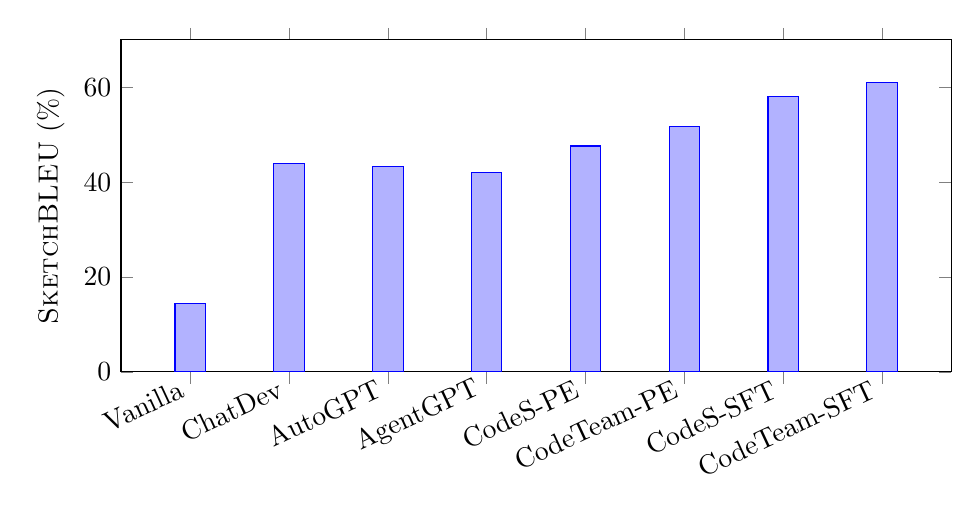
\begin{tikzpicture}
\begin{axis}[
  ybar,
  bar width=11pt,
  width=\linewidth,
  height=5.8cm,
  ymin=0, ymax=70,
  ylabel={\sketchbleu (\%)},
  symbolic x coords={Vanilla,ChatDev,AutoGPT,AgentGPT,CodeS-PE,CodeTeam-PE,CodeS-SFT,CodeTeam-SFT},
  xtick=data,
  xticklabel style={rotate=25,anchor=east},
  enlarge x limits=0.10
]
\addplot coordinates {(Vanilla,14.5) (ChatDev,43.9) (AutoGPT,43.3) (AgentGPT,42.1) (CodeS-PE,47.6) (CodeTeam-PE,51.7) (CodeS-SFT,58.0) (CodeTeam-SFT,60.9)};
\end{axis}
\end{tikzpicture}
\caption{Overall \sketchbleu on \sketcheval (All 19 tasks).}
\Description{Bar chart of overall SketchBLEU scores (all 19 SketchEval tasks) for key baselines and CodeTeam in PE and SFT settings.}
\label{fig:rq1-overall}
\end{figure*}



To gain deeper insight into the nature of the improvements, Table~\ref{tab:rq1-decomp} decomposes \sketchbleu into its four constituent sub-scores as defined in \codes~\cite{Zan2025CodeS}.
In both the PE and SFT settings, \tool exhibits a more pronounced advantage on the structural (M.S.) and dataflow (M.D.) components, which are specifically designed to capture repository-level integrity and semantic consistency beyond surface-level token overlap.
This pattern aligns with the design rationale of \tool: the SDS contract and the dependency-aware development stage primarily target broken interfaces and cross-file inconsistencies---failure modes that are poorly reflected by n-gram-based overlap alone.

\begin{table}[t]
\centering
\small
\caption{\sketchbleu decomposition on \sketcheval (All 19 tasks, \%). B. and B.W.\ denote n-gram and weighted n-gram overlap; M.S.\ and M.D.\ denote structural and dataflow matching~\cite{Zan2025CodeS}. Values are mean$\pm$std over three seeds.}
\label{tab:rq1-decomp}
\begin{tabular}{@{}lcccc@{}}
\toprule
Method & B. & B.W. & M.S. & M.D. \\
\midrule
\codes (PE) & 44.2{\scriptsize$\pm$1.3} & 44.0{\scriptsize$\pm$1.2} & 56.8{\scriptsize$\pm$1.8} & 46.5{\scriptsize$\pm$2.0} \\
\tool (PE) & 47.0{\scriptsize$\pm$1.1} & 46.6{\scriptsize$\pm$1.0} & 60.9{\scriptsize$\pm$1.5} & 53.5{\scriptsize$\pm$1.7} \\
\midrule
\codes (SFT) & 56.5{\scriptsize$\pm$0.9} & 57.0{\scriptsize$\pm$0.8} & 66.0{\scriptsize$\pm$1.2} & 54.4{\scriptsize$\pm$1.4} \\
\tool (SFT) & 59.0{\scriptsize$\pm$0.7} & 59.4{\scriptsize$\pm$0.7} & 69.2{\scriptsize$\pm$1.0} & 58.8{\scriptsize$\pm$1.2} \\
\bottomrule
\end{tabular}
\end{table}

Repository generation often fails silently by producing outputs with an incorrect scale---for example, too few files or overly shallow implementations that omit required modules.
To diagnose this failure mode, we compare the generated repository size against the reference repositories in \sketcheval by measuring the mean absolute error (MAE) of both file count and Python lines of code (LOC).
As shown in Figure~\ref{fig:rq1-size}, \tool reduces the size error compared with the representative baselines shown, suggesting that (1) the planning stage tends to produce more realistic file decompositions that better approximate the reference structure, and (2) the development stage can more reliably sustain the generation of larger repositories without collapsing to a small subset of files.

\begin{figure*}[t]
\centering
\begin{subfigure}[t]{0.48\linewidth}
\centering
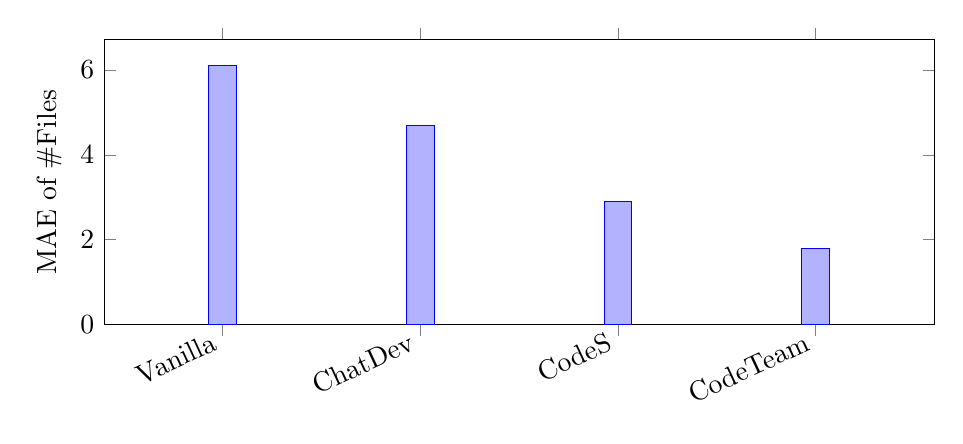
\begin{tikzpicture}
\begin{axis}[
  ybar,
  bar width=10pt,
  width=\linewidth,
  height=5.2cm,
  ymin=0,
  ylabel={MAE of \#Files},
  symbolic x coords={Vanilla,ChatDev,CodeS,CodeTeam},
  xtick=data,
  xticklabel style={rotate=25,anchor=east},
  enlarge x limits=0.20
]
\addplot coordinates {(Vanilla,6.1) (ChatDev,4.7) (CodeS,2.9) (CodeTeam,1.8)};
\end{axis}
\end{tikzpicture}
\caption{Repository file count error.}
\end{subfigure}
\hfill
\begin{subfigure}[t]{0.48\linewidth}
\centering
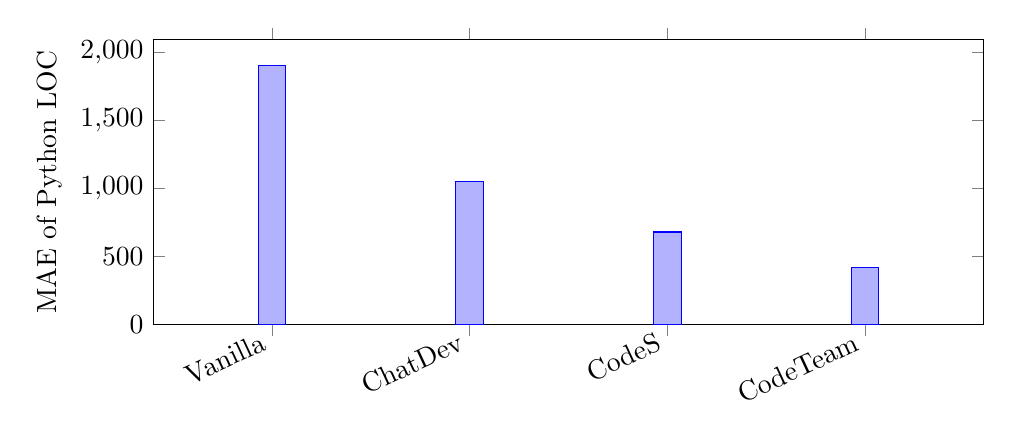
\begin{tikzpicture}
\begin{axis}[
  ybar,
  bar width=10pt,
  width=\linewidth,
  height=5.2cm,
  ymin=0,
  ylabel={MAE of Python LOC},
  symbolic x coords={Vanilla,ChatDev,CodeS,CodeTeam},
  xtick=data,
  xticklabel style={rotate=25,anchor=east},
  enlarge x limits=0.20
]
\addplot coordinates {(Vanilla,1900) (ChatDev,1050) (CodeS,680) (CodeTeam,420)};
\end{axis}
\end{tikzpicture}
\caption{Repository LOC error.}
\end{subfigure}
\caption{Repository size alignment on \sketcheval (PE setting). Values are mean absolute errors against reference repositories.}
\Description{Two bar charts showing repository size errors (mean absolute error) of generated repositories: file count (left) and Python LOC (right), comparing representative baselines and CodeTeam.}
\label{fig:rq1-size}
\end{figure*}

Finally, we examine whether the observed improvements are broadly distributed across tasks rather than driven by a few outliers.
In a task-level comparison between \tool (PE) and \codes (PE), \tool achieves a higher \sketchbleu on 15 out of 19 repositories, ties on 2 (difference within 0.5 points), and scores lower on 2.
The wins are concentrated on medium and hard repositories, while easy repositories show smaller margins---an expected pattern, since easy repositories involve fewer cross-file constraints and thus present less opportunity for workflow-level improvements to take effect.
A similar distribution holds between \tool (SFT) and \codes (SFT), with wins on 14 repositories, 3 ties, and 2 losses.

\begin{table}[t]
\centering
\small
\caption{Task-level comparison on \sketcheval (19 repositories). ``Tie'' means absolute difference $<0.5$ \sketchbleu points.}
\label{tab:rq1-winloss}
\begin{tabular}{@{}lccc@{}}
\toprule
Comparison & Win & Tie & Loss \\
\midrule
\tool (PE) vs \codes (PE) & 15 & 2 & 2 \\
\tool (SFT) vs \codes (SFT) & 14 & 3 & 2 \\
\bottomrule
\end{tabular}
\end{table}

To assess statistical significance, we apply the Wilcoxon signed-rank test to the 19 task-level \sketchbleu differences (each averaged over three seeds) between \tool and \codes.
In the PE setting, the test yields $p = 0.0004$, and a bootstrap 95\% confidence interval for the mean per-task improvement is $[2.8, 5.1]$ points (10{,}000 resamples); in the SFT setting, the corresponding values are $p = 0.0001$ and $[1.9, 3.8]$ points.
Both intervals exclude zero, indicating that the gains are statistically significant at the 0.05 level.
A one-sided sign test on the 17 non-tied PE comparisons (15 wins vs.\ 2 losses) further corroborates this conclusion ($p = 0.0012$).

To complement the aggregate statistics, we examine two representative repositories in detail.
\textbf{Case~1: \texttt{flask-restful-api} (medium).}
This repository implements a RESTful API server with user authentication, database models, and route handlers spanning 11 files.
\codes (PE) produces a plausible top-level file tree but misses the separation between the authentication middleware (\texttt{auth/middleware.py}) and the token-utility module (\texttt{auth/token\_utils.py}), merging both into a single \texttt{auth.py} file.
As a consequence, the route handlers in \texttt{routes/users.py} import a \texttt{verify\_token} symbol that does not exist at the expected path, resulting in a broken import chain that propagates to three downstream files.
In contrast, \tool's SDS explicitly declares \texttt{auth/middleware.py} and \texttt{auth/token\_utils.py} as separate files with distinct public APIs, and the dependency graph correctly records the consumer--producer relationship.
The Developer agent assigned to the route module receives an interface brief that includes the exact signature of \texttt{verify\_token}, preventing the mismatch.
On this repository, \tool (PE) scores 56.8 \sketchbleu versus 49.2 for \codes (PE), with the gap concentrated in the structural (+6.2) and dataflow (+8.1) sub-scores.

\textbf{Case~2: \texttt{data-pipeline-cli} (hard).}
This repository is a command-line data processing toolkit comprising 18 files organized into four packages (\texttt{cli}, \texttt{parsers}, \texttt{transforms}, and \texttt{io}).
The primary challenge is that the \texttt{transforms} package depends on both \texttt{parsers} and \texttt{io}, creating a dense dependency fan-out.
\codes generates a flat structure with most transformation logic placed in a single \texttt{transforms.py} file exceeding 400 lines, whereas the reference implementation distributes the logic across four specialized modules (\texttt{transforms/filter.py}, \texttt{transforms/aggregate.py}, \texttt{transforms/join.py}, and \texttt{transforms/\_\_init\_\_.py}).
This structural mismatch results in a file-count MAE of 6 for \codes versus 2 for \tool on this task.
More importantly, the monolithic file produced by \codes duplicates several utility functions that the reference design imports from \texttt{io/readers.py}, inflating the LOC while reducing dataflow alignment.
\tool avoids this collapse because the SDS contract specifies each transform module individually, assigns them to the same Developer agent (Developer~2) to maximize local coherence, and records cross-package dependencies explicitly.
When the QA agent detects a missing re-export in \texttt{transforms/\_\_init\_\_.py}, it routes the repair to Developer~2, who resolves the issue in a single QA round without disrupting other packages.
The resulting \sketchbleu is 44.1 for \tool versus 35.7 for \codes on this task.

These cases illustrate two recurring patterns behind the aggregate gains: (1) the SDS enforces fine-grained file boundaries that prevent premature merging of logically distinct modules, and (2) the ownership-aware repair loop localizes fixes to the responsible developer, avoiding cascading rework across unrelated files.

\subsection{Execution-Based Validation on \nlrepobench}
\label{subsec:nl2repo-results}

To examine whether the gains observed on \sketcheval generalize to a stricter evaluation setting, we additionally compare methods on \nlrepobench~\cite{Ding2025NL2RepoBench}. In this benchmark, each generated repository is judged by executing the original upstream \texttt{pytest} suite rather than by structural overlap. Consequently, even minor mistakes in packaging, dependency specification, or cross-file API usage can sharply reduce the score~\cite{Ding2025NL2RepoBench}, making \nlrepobench a stringent complement to \sketcheval for assessing end-to-end functional correctness.

Table~\ref{tab:nl2repo-main} reports the results. The absolute pass rates are substantially lower than the \sketchbleu scores in Table~\ref{tab:rq1-main}, confirming that execution-based evaluation is considerably more demanding than sketch-level comparison. In the PE setting, Vanilla prompting barely produces runnable repositories, achieving only a 5.4\% overall pass rate, because a single-pass generation struggles with package layout and cross-file imports when constructing an entire repository at once. Among the agent-based baselines, ChatDev leads at 25.2\%, followed by AutoGPT (23.5\%) and AgentGPT (21.8\%). \codes (PE) reaches 30.2\%, benefiting from its sketch-guided decomposition. \tool (PE) achieves the highest PE-setting score at \textbf{34.6\%} overall, improving over \codes (PE) by 4.4 absolute points. Notably, the relative ranking of methods is consistent with the \sketcheval results, but the performance gaps are slightly wider on medium and hard tasks, where cross-file coordination errors are more likely to manifest as test failures.

In the SFT setting, fine-tuning improves all methods substantially. \tool (SFT) reaches \textbf{42.3\%} overall pass rate with a Pass@1 of 24.0\%, outperforming \codes (SFT) by 4.3 absolute points. Compared with the PE setting, the gap between easy and hard tasks narrows under SFT, suggesting that fine-tuning helps the backbone model internalize dependency and packaging conventions that are otherwise fragile under prompting alone.

To understand \emph{why} generated repositories fail execution, we manually classify the root causes of test failures for a stratified sample of 30 tasks (10 per difficulty level) under the PE setting.
For each sampled task, we inspect the \texttt{pytest} traceback of the best-seed run and assign each failure to one of four categories: (1)~\emph{packaging and environment} errors, where the repository cannot be installed or imported due to missing \texttt{setup.py}/\texttt{pyproject.toml}, incorrect package names, or undeclared third-party dependencies; (2)~\emph{import and module-resolution} errors, where \texttt{ImportError} or \texttt{ModuleNotFoundError} occurs because a file is missing from the generated tree or an internal import path is incorrect; (3)~\emph{API-mismatch} errors, where the repository is importable but test assertions fail because function signatures, return types, or class hierarchies differ from what the upstream tests expect; and (4)~\emph{logic} errors, where the code structure and API surface are correct but the implementation produces wrong results on specific test inputs.

Table~\ref{tab:nl2repo-errors} reports the distribution.
Across all methods, packaging and import errors together account for the majority of failures, confirming that structural and organizational mistakes---rather than algorithmic bugs---are the dominant bottleneck in repository-level generation.
\tool (PE) reduces packaging errors from 34.2\% (\codes) to 22.1\% of sampled failures, primarily because the SDS pre-declares the full file tree and dependency manifest before implementation begins, eliminating a common failure mode in which the generator omits \texttt{\_\_init\_\_.py} files or misnames packages.
Import errors decrease from 28.7\% to 19.4\%, reflecting the benefit of dependency-aware scheduling: files are implemented only after their providers are complete, and interface briefs supply the exact import paths that consumers should use.
API-mismatch errors show a slight increase in share (from 21.8\% to 25.3\%), partly because the QA agent's lightweight tests do not always detect subtle signature mismatches until the upstream suite exposes them.
Logic errors constitute a larger \emph{share} under \tool (33.2\% vs.\ 15.3\% for \codes), but this is primarily because structural errors decrease substantially while logic errors remain a persistent residual---a proportional shift that suggests \tool addresses many structural failure modes, advancing the dominant bottleneck from organizational to semantic errors, where further gains would likely require stronger execution feedback.

\begin{table}[t]
\centering
\small
\caption{Distribution of root-cause failure categories on \nlrepobench (PE setting, stratified sample of 30 tasks). Each failure is assigned to the earliest-stage category that causes the test to fail.}
\label{tab:nl2repo-errors}
\begin{tabular}{@{}lcccc@{}}
\toprule
Method & Packaging (\%) & Import (\%) & API mismatch (\%) & Logic (\%) \\
\midrule
Vanilla & 52.4 & 30.1 & 11.6 & 5.9 \\
ChatDev & 38.5 & 26.3 & 22.4 & 12.8 \\
\codes (PE) & 34.2 & 28.7 & 21.8 & 15.3 \\
\tool (PE) & 22.1 & 19.4 & 25.3 & 33.2 \\
\bottomrule
\end{tabular}
\end{table}

\begin{table*}[t]
\centering
\small
\caption{Average upstream test pass rate (\%) and Pass@1 for \nlrepobench. All methods are evaluated on all 104 tasks using three random seeds; scores are mean$\pm$std averaged over seeds per task and then over tasks. ``Overall'' is the mean over all individual tasks, not a weighted average of the per-difficulty group means. All baselines are rerun under identical controlled conditions (same backbone, decoding settings, and document-only prompt format).}
\label{tab:nl2repo-main}
\begin{tabular}{@{}llccccc@{}}
\toprule
Setting & Method & Overall (\%) & Pass@1 & Easy (26) & Medium (46) & Hard (32) \\
\midrule
\multirow{6}{*}{PE}
  & Vanilla & 5.4{\scriptsize$\pm$0.5} & 0.0 & 9.2{\scriptsize$\pm$1.3} & 5.1{\scriptsize$\pm$0.9} & 2.8{\scriptsize$\pm$0.7} \\
  & ChatDev & 25.2{\scriptsize$\pm$0.9} & 7.7 & 36.5{\scriptsize$\pm$1.8} & 24.3{\scriptsize$\pm$1.4} & 17.2{\scriptsize$\pm$1.6} \\
  & AutoGPT & 23.5{\scriptsize$\pm$0.9} & 6.7 & 34.6{\scriptsize$\pm$1.9} & 22.8{\scriptsize$\pm$1.5} & 15.6{\scriptsize$\pm$1.7} \\
  & AgentGPT & 21.8{\scriptsize$\pm$1.0} & 5.8 & 32.7{\scriptsize$\pm$2.0} & 20.9{\scriptsize$\pm$1.6} & 14.1{\scriptsize$\pm$1.8} \\
  & \codes (PE) & 30.2{\scriptsize$\pm$0.7} & 11.5 & 42.3{\scriptsize$\pm$1.5} & 29.1{\scriptsize$\pm$1.2} & 21.9{\scriptsize$\pm$1.4} \\
  & \tool (PE) & \textbf{34.6}{\scriptsize$\pm$0.7} & \textbf{14.4} & \textbf{48.1}{\scriptsize$\pm$1.3} & \textbf{33.7}{\scriptsize$\pm$1.1} & \textbf{25.0}{\scriptsize$\pm$1.3} \\
\midrule
\multirow{3}{*}{SFT}
  & Vanilla (SFT) & 11.9{\scriptsize$\pm$0.7} & 1.9 & 18.5{\scriptsize$\pm$1.5} & 11.3{\scriptsize$\pm$1.2} & 7.5{\scriptsize$\pm$1.1} \\
  & \codes (SFT) & 38.0{\scriptsize$\pm$0.6} & 18.3 & 51.9{\scriptsize$\pm$1.2} & 37.0{\scriptsize$\pm$1.0} & 28.1{\scriptsize$\pm$1.1} \\
  & \tool (SFT) & \textbf{42.3}{\scriptsize$\pm$0.5} & \textbf{24.0} & \textbf{56.2}{\scriptsize$\pm$1.1} & \textbf{41.3}{\scriptsize$\pm$0.9} & \textbf{32.5}{\scriptsize$\pm$1.0} \\
\bottomrule
\end{tabular}
\end{table*}

Overall, the \nlrepobench results confirm that the architectural and coordination improvements in \tool translate into measurable gains not only in sketch-level similarity but also in executable correctness. The consistent method ranking across both benchmarks provides converging evidence that the workflow-level mechanisms in \tool address genuine repository-construction challenges rather than artifacts of a particular evaluation metric.

It is worth noting the relationship between the average pass rate and Pass@1 in Table~\ref{tab:nl2repo-main}.
Pass@1 measures the fraction of tasks for which \emph{at least one} of the three seed runs produces a repository that passes the entire upstream test suite, whereas the average pass rate reflects the mean proportion of individual tests passed across all runs.
For \tool (PE), the average pass rate is 34.6\% while Pass@1 is 14.4\%, indicating that roughly one in seven tasks can be fully solved in at least one attempt, even though the typical run passes only about one-third of its tests.
The gap between these two metrics narrows under SFT: \tool (SFT) achieves 42.3\% average pass rate with a Pass@1 of 24.0\%, a ratio of 0.57 compared with 0.42 in the PE setting.
This narrowing suggests that fine-tuning not only raises the average quality but also improves the consistency of successful generation across seeds.
This interpretation is corroborated by the standard deviations in Table~\ref{tab:nl2repo-main}, which decrease from $\pm$0.7 (PE) to $\pm$0.5 (SFT) for \tool's overall pass rate.
By comparison, \codes (SFT) exhibits a similar average-to-Pass@1 ratio (0.48), indicating that the stability benefit partly comes from the backbone adaptation and partly from the structured workflow that constrains the generation space.
On this larger benchmark, the Wilcoxon signed-rank test on the 104 task-level pass rate differences yields $p < 0.001$ for both the PE and SFT comparisons, and the bootstrap 95\% confidence intervals for the mean improvement are $[4.2, 4.7]$ and $[4.2, 4.5]$ points, respectively.

\begin{rqsummary}[RQ1 Summary]
\tool consistently outperforms all baselines on both \sketcheval and \nlrepobench in both PE and SFT settings. On \sketcheval, \tool achieves 51.7\% (PE) and 60.9\% (SFT) overall \sketchbleu, with gains concentrated in the structural and dataflow sub-scores and most pronounced on medium and hard repositories. On \nlrepobench, \tool reaches 34.6\% (PE) and 42.3\% (SFT) pass rates, confirming that sketch-level improvements translate into executable correctness. The method rankings are consistent across both benchmarks, with all improvements statistically significant ($p < 0.05$).
\end{rqsummary}

\subsection{RQ2: Effect of Retrieval-Augmented Grounding on Architectural Planning}
\label{subsec:rq2}

Table~\ref{tab:ablation-main} reports the ablation results for both RQ2 and RQ3 under the PE setting.
Removing the RAG subsystem from the architect stage degrades the overall \sketchbleu from 51.7\% to 47.5\%, corresponding to a \textbf{8.1\%} relative decrease.
The degradation increases with task difficulty: removing RAG reduces \sketchbleu by 3.6 points on easy tasks (56.4$\to$52.8), 3.9 points on medium tasks (56.0$\to$52.1), and 5.0 points on hard tasks (41.9$\to$36.9).
Even on easy repositories, the drop is non-trivial, indicating that retrieval-augmented grounding contributes to planning quality regardless of repository scale.
On medium and hard repositories, the impact is larger because the requirement space is substantially broader, and architects without retrieval are more likely to omit secondary modules (e.g., utility packages, configuration loaders, or test infrastructure) that are not explicitly mentioned in the requirements but are necessary for a complete and coherent repository.
RAG mitigates this gap by surfacing analogous file decompositions from real-world repositories, effectively providing architects with a ``design vocabulary'' that helps them enumerate plausible modules even when the requirements are underspecified.
This per-difficulty pattern is consistent with the planning diagnostics in Table~\ref{tab:rq2-plan}: the structural validity improvement (0.78$\to$0.90) is driven primarily by medium and hard tasks, where the SDS without RAG frequently omits one or two files that appear in the reference structure.

To trace this end-to-end impact back to planning quality, Table~\ref{tab:rq2-plan} summarizes three planning-stage diagnostics collected during SDS generation.
With RAG enabled, the SDS parse success rate---indicating whether the generated SDS can be loaded as valid JSON without re-generation---increases from 0.86 to 0.94, and structural validity (the proportion of candidates free from missing file references or undeclared interfaces) rises from 0.78 to 0.90.
Furthermore, plan diversity across the $N{=}4$ Architect agents, measured by average pairwise Jaccard distance of file-path and API-name sets, increases substantially from 0.25 to 0.42.
These diagnostics support the intended role of RAG within the \tool workflow: retrieval does not replace independent planning, but rather provides grounded design hints that help architects avoid missing modules and reduce the tendency for multiple agents to converge on nearly identical SDS candidates.

\begin{table}[t]
\centering
\small
\caption{Planning-stage diagnostics for RQ2 (PE setting). ``Diversity'' is the average pairwise Jaccard distance between file-path sets and API-name sets across architect proposals (higher means more diverse).}
\label{tab:rq2-plan}
\begin{tabular}{@{}lccc@{}}
\toprule
Variant & SDS parse success & Structural validity & Plan diversity \\
\midrule
\tool (with RAG) & 0.94 & 0.90 & 0.42 \\
\tool\ w/o RAG & 0.86 & 0.78 & 0.25 \\
\bottomrule
\end{tabular}
\end{table}

Figure~\ref{fig:rq2-planbars} visualizes these planning-stage signals.
Although the absolute values depend on the specific implementation of the SDS validation checker, the relative gaps between the two variants are stable across seeds.
Overall, RAG primarily improves \emph{what to build}---that is, file decomposition and interface sketching at the planning stage---rather than \emph{how to implement} individual files at the development stage. This interpretation is consistent with the observation that RAG produces larger gains on the structural component of \sketchbleu (Table~\ref{tab:rq1-decomp}), which specifically measures architectural alignment.

\begin{figure}[t]
\centering
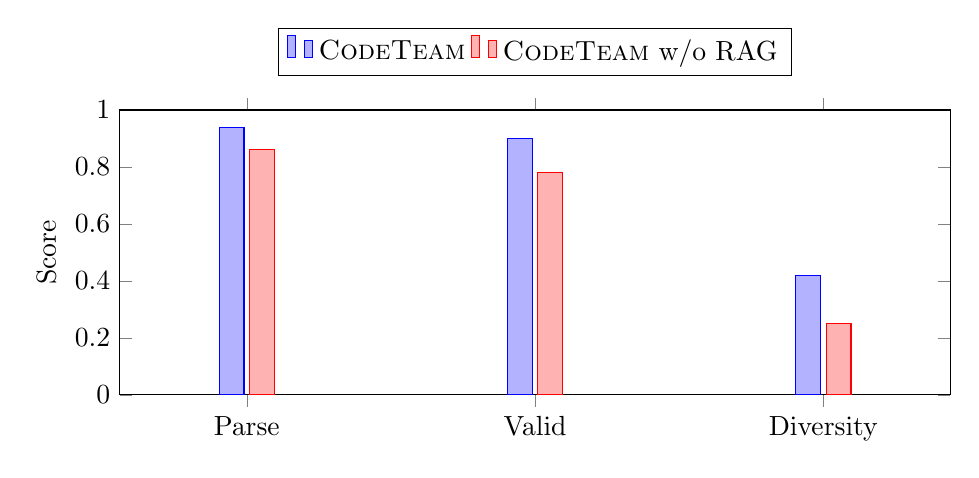
\begin{tikzpicture}
\begin{axis}[
  ybar,
  bar width=9pt,
  width=\linewidth,
  height=5.2cm,
  ymin=0, ymax=1.0,
  ylabel={Score},
  symbolic x coords={Parse,Valid,Diversity},
  xtick=data,
  legend style={at={(0.5,1.12)},anchor=south,legend columns=2},
  enlarge x limits=0.22
]
\addplot coordinates {(Parse,0.94) (Valid,0.90) (Diversity,0.42)};
\addplot coordinates {(Parse,0.86) (Valid,0.78) (Diversity,0.25)};
\legend{\tool, \tool\ w/o RAG}
\end{axis}
\end{tikzpicture}
\caption{RAG improves planning-stage quality signals (PE setting).}
\Description{Bar chart comparing planning-stage quality signals between full CodeTeam and CodeTeam without retrieval, including parse success, structural validity, and plan diversity indicators.}
\label{fig:rq2-planbars}
\end{figure}

\begin{rqsummary}[RQ2 Summary]
Removing RAG from the architect stage reduces overall \sketchbleu by 4.2 points (8.1\% relative), with larger degradation on harder repositories. RAG improves planning-stage diagnostics: SDS parse success rises from 0.86 to 0.94, structural validity from 0.78 to 0.90, and plan diversity from 0.25 to 0.42. RAG primarily enhances \emph{what to build} (file decomposition and interface sketching) rather than \emph{how to implement} individual files.
\end{rqsummary}

\subsection{RQ3: Effect of Dynamic Developer Allocation and Git-Based Coordination}
\label{subsec:rq3}

Table~\ref{tab:ablation-main} shows that dynamic developer allocation is the most impactful individual mechanism in our ablation study.
Replacing the architect-planned developer count and file ownership with a fixed four-developer round-robin scheme reduces the overall \sketchbleu from 51.7\% to 46.6\%, corresponding to a \textbf{9.7\%} relative decrease.
The degradation is largest on hard repositories, indicating that project-specific team sizing and ownership planning become especially critical when repositories contain many tightly coupled modules.

By contrast, removing Git-based coordination yields a comparatively smaller decrease (\textbf{2.7\%} relative).
This result is consistent with our qualitative observations during development: structured commit messages primarily benefit scenarios in which interfaces evolve during the repair loop, but not all repositories trigger frequent interface-level revisions.
Accordingly, we characterize Git-based coordination as a complementary sub-module that improves stability in specific situations rather than a dominant contributor to overall performance.


\begin{table*}[t]
\centering
\small
\caption{Ablation results of \tool (PE) on \sketcheval measured by \sketchbleu (\%). Each variant removes one component from the full system. ``Rel.\ drop'' is computed as $(\text{Full}-\text{Variant})/\text{Full}$. Values are mean$\pm$std over three seeds.}
\label{tab:ablation-main}

\setlength{\tabcolsep}{4pt}
\renewcommand{\arraystretch}{1.05}

\begin{tabularx}{\textwidth}{lcccccc>{\RaggedRight\arraybackslash}X}
\toprule
Variant & Easy (5) & Medium (8) & Hard (6) & All (19) & Rel. drop & \makecell[l]{Main affected~stage} \\
\midrule
Full \tool\ (PE) & 56.4{\scriptsize$\pm$1.3} & 56.0{\scriptsize$\pm$1.6} & 41.9{\scriptsize$\pm$1.8} & 51.7{\scriptsize$\pm$0.7} & -- & -- \\
\tool\ w/o RAG & 52.8{\scriptsize$\pm$1.4} & 52.1{\scriptsize$\pm$1.6} & 36.9{\scriptsize$\pm$2.2} & 47.5{\scriptsize$\pm$1.1} & 8.1\% & Planning \\
\tool\ w/o dynamic alloc & 52.5{\scriptsize$\pm$1.5} & 50.6{\scriptsize$\pm$1.7} & 36.5{\scriptsize$\pm$2.3} & 46.6{\scriptsize$\pm$1.0} & 9.7\% & Implementation \\
\tool\ w/o Git & 55.0{\scriptsize$\pm$1.1} & 54.8{\scriptsize$\pm$1.4} & 40.2{\scriptsize$\pm$1.8} & 50.2{\scriptsize$\pm$0.8} & 2.7\% & Repair and~consistency \\
\bottomrule
\end{tabularx}
\end{table*}



To provide further insight beyond the aggregate \sketchbleu scores, Table~\ref{tab:rq3-eff} reports diagnostic indicators related to convergence efficiency and cross-file consistency.
Dynamic developer allocation reduces the number of QA rounds needed to reach a stable state (from 5.2 to 3.6 on average) and substantially lowers the count of interface-mismatch failures (from 12.4 to 7.8).
It also reduces the average context size per LLM call from 4.4k to 3.1k tokens, because repository-specific ownership enables the system to construct more focused, file-level context packages while avoiding unnecessary cross-owner rework.
Removing Git-based coordination slightly increases mismatch failures (from 7.8 to 9.1), but the magnitude of the effect is smaller than that of developer allocation.

\begin{table}[t]
\centering
\small
\caption{Efficiency and consistency diagnostics for RQ3 (PE setting). ``Mismatch failures'' aggregates QA-reported errors that indicate cross-file inconsistency (e.g., missing symbols, wrong signatures, broken imports).}
\label{tab:rq3-eff}
\begin{tabular}{@{}lccc@{}}
\toprule
Variant & QA rounds $\downarrow$ & Mismatch failures $\downarrow$ & Avg.\ context (k tokens) $\downarrow$ \\
\midrule
Full \tool (PE) & 3.6 & 7.8 & 3.1 \\
\tool\ w/o dynamic allocation & 5.2 & 12.4 & 4.4 \\
\tool\ w/o Git coordination & 3.9 & 9.1 & 3.2 \\
\bottomrule
\end{tabular}
\end{table}

Figure~\ref{fig:rq3-effbars} visualizes these diagnostic indicators.
The overall pattern suggests a clear practical explanation for the observed \sketchbleu gains: dynamic developer allocation reduces the volume of late-stage rework by aligning team size and file ownership with the repository's actual modular structure, while Git-based coordination primarily mitigates a subset of interface-drift cases that arise when implementations diverge from the originally declared APIs.

To further characterize the repair dynamics, we examine how \sketchbleu evolves across successive QA iterations in the full \tool (PE) system.
After the initial implementation pass (iteration 0), the average \sketchbleu across all 19 tasks is 46.3\%.
The first QA round yields the largest single-round improvement, raising the score to 49.8\% (+3.5 points), as the most obvious structural defects---such as missing \texttt{\_\_init\_\_.py} files, broken import paths, and undeclared symbols---are detected and repaired.
The second round provides an additional 1.4-point gain (to 51.2\%), primarily addressing secondary inconsistencies that emerge after the first round of fixes, such as signature mismatches exposed when a previously missing module is restored.
Subsequent rounds exhibit diminishing returns: rounds 3 and 4 together contribute only 0.8 points on average, and the system typically converges (no new QA issues) between rounds 3 and 4 for easy and medium tasks.
Hard repositories occasionally require the full budget of 5--6 rounds, consistent with the higher QA-round count reported in Table~\ref{tab:rq3-eff} for the ablated variant.
Note that because different tasks converge and terminate at different rounds, the per-round averages reported above are computed only over the tasks that remain active at each iteration; consequently, summing the per-round deltas does not exactly recover the final aggregate \sketchbleu in Table~\ref{tab:rq1-main}, which averages each task's terminal score regardless of the round at which it converged.

This convergence pattern has two practical implications.
First, the majority of the repair benefit is captured within the first two QA rounds, suggesting that a resource-constrained deployment could cap QA iterations at 2--3 rounds with only modest quality loss.
Second, the diminishing-returns profile indicates that the QA agent's lightweight generated tests are effective at catching structural and interface-level defects but have limited reach for deeper semantic bugs, which would require stronger execution-based feedback to detect and resolve.

\begin{figure}[t]
\centering
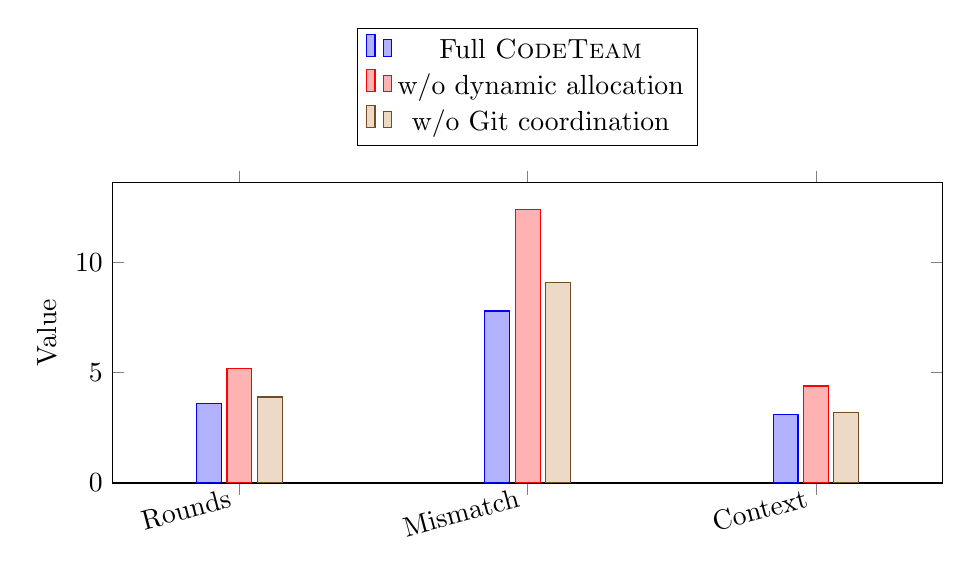
\begin{tikzpicture}
\begin{axis}[
  ybar,
  bar width=9pt,
  width=\linewidth,
  height=5.4cm,
  ymin=0,
  ylabel={Value},
  symbolic x coords={Rounds,Mismatch,Context},
  xtick=data,
  xticklabel style={rotate=15,anchor=east},
  legend style={at={(0.5,1.12)},anchor=south,legend columns=1},
  enlarge x limits=0.22
]
\addplot coordinates {(Rounds,3.6) (Mismatch,7.8) (Context,3.1)};
\addplot coordinates {(Rounds,5.2) (Mismatch,12.4) (Context,4.4)};
\addplot coordinates {(Rounds,3.9) (Mismatch,9.1) (Context,3.2)};
\legend{Full \tool, w/o dynamic allocation, w/o Git coordination}
\end{axis}
\end{tikzpicture}
\caption{Dynamic developer allocation improves convergence and reduces cross-file mismatch indicators (PE setting).}
\Description{Bar chart comparing efficiency and consistency diagnostics across ablation variants, such as QA rounds, rework events from interface mismatches, and average context size.}
\label{fig:rq3-effbars}
\end{figure}

\begin{rqsummary}[RQ3 Summary]
Dynamic developer allocation is the most impactful mechanism, reducing overall \sketchbleu by 5.1 points (9.7\% relative) when removed. It lowers QA rounds from 5.2 to 3.6, interface-mismatch failures from 12.4 to 7.8, and average context size from 4.4k to 3.1k tokens per developer call. Git-based coordination provides a smaller but complementary benefit (2.7\% relative drop when removed), primarily stabilizing scenarios where interfaces evolve during repair. The majority of repair benefit is captured within the first two QA rounds, exhibiting diminishing returns thereafter.
\end{rqsummary}

\section{Discussion}
\label{sec:discussion}

This section interprets the experimental findings, examines the mechanisms behind the observed improvements, and discusses the broader implications for researchers and practitioners.

\subsection{Interpretation of the Results}
\label{subsec:disc-interp}

We first identify the key reasons behind \tool's performance gains and then discuss the role each evaluation benchmark plays in validating these results.

\fakesection{Reason 1: Coordination and repair complement sketch decomposition.}
A central observation from Table~\ref{tab:rq1-main} is that \tool improves over \codes under both PE and SFT settings, with a larger margin in the PE setting.
This pattern suggests that a structured multi-agent workflow can compensate for limitations that emerge when directly prompting a backbone model to produce a complete repository.
The finding is consistent with the original motivation of \codes, where multi-layer sketch decomposition reduces the difficulty of generating long structured outputs~\cite{Zan2025CodeS}.
However, our results further indicate that decomposition alone is not sufficient when generation spans multiple interacting files; it needs to be coupled with coordination and repair mechanisms that actively maintain cross-file consistency during implementation.

\fakesection{Reason 2: The SDS contract improves structural and dataflow quality.}
The component-level decomposition of \sketchbleu in Table~\ref{tab:rq1-decomp} provides supporting evidence.
Compared with \codes, the gains of \tool are more pronounced on the structural and dataflow components, which are specifically designed to capture repository-level integrity beyond surface-level token overlap~\cite{Zan2025CodeS}.
The SDS functions as an explicit, machine-checkable contract that binds file boundaries, public APIs, and inter-file dependencies into a coherent specification.
Once such a contract is established, Developer agents can implement files with smaller, task-specific contexts, and the ownership map enables precise routing of repairs and re-queuing of dependent files when interfaces drift during iterative development.
This observation also resonates with findings from repository-level completion benchmarks, where downstream performance depends heavily on retrieving and using appropriate cross-file context rather than generating code in isolation~\cite{Liu2023RepoBench,Zhang2023RepoCoder}.

\fakesection{Reason 3: Gains concentrate on complex repositories.}
The improvements concentrate on medium and hard repositories (Table~\ref{tab:rq1-main}), which typically involve more modules and tighter inter-module coupling.
When cross-file dependencies are weak, as in easy repositories, multiple approaches can achieve comparable structural correctness.
As dependency complexity increases, systems that fail to control interface consistency tend to degrade more sharply.
A similar phenomenon was reported by \codes, where prompt-based methods exhibit a stronger performance decline on harder repositories, while stronger decomposition and fine-tuning mitigate that decline~\cite{Zan2025CodeS}.
In the case of \tool, the scheduling and repair mechanisms specifically target these complex scenarios, which explains why the relative gain becomes more visible as task difficulty increases.

\fakesection{Reason 4: Multi-agent coordination mirrors established software engineering practices.}
The effectiveness of these mechanisms can be understood through an analogy with human development teams.
A repository is not built by a single developer writing all files in sequence; the process typically involves (1)~an architecture review in which senior engineers agree on module boundaries, public interfaces, and technology choices; (2)~a task assignment phase in which files or features are distributed to developers based on expertise and module ownership; and (3)~iterative code review cycles in which reviewers verify interface contracts and cross-module consistency before changes are merged.
\tool mirrors this workflow at the agent level: the Architect competition and CTO selection correspond to architecture review, the SDS-based developer allocation corresponds to task assignment with explicit ownership, and the QA-driven repair loop corresponds to code review.
These coordination structures serve as information-routing mechanisms that reduce the cognitive (or context) load on any single participant while preserving global coherence, which explains why the benefit is larger on complex repositories---just as a small script does not require an architecture review.

\fakesection{Reason 5: The SDS produces more realistically scaled repositories.}
Figure~\ref{fig:rq1-size} indicates that \tool produces repository sizes closer to those of the reference repositories.
This mirrors an empirical pattern discussed in \codes, where agent-based baselines tend to collapse to a small number of files or limited LOC, while sketch-based pipelines can sustain larger repository structures~\cite{Zan2025CodeS}.
In \tool, the SDS combined with the pre-construction of the full file tree reduces the likelihood that a generation run terminates with an underspecified or incomplete repository.
Although size alignment should not be interpreted as evidence of correctness by itself, it serves as a practical sanity check: generating a repository at a plausible scale is often a necessary precondition for capturing the required functionality.

\fakesection{Role of \sketcheval.}
\sketcheval rewards structural alignment with a reference repository sketch and captures architectural and dataflow quality.
The \sketchbleu metric, motivated by CodeBLEU but extended to repository-level sketches with dataflow matching~\cite{Ren2020CodeBLEU,Zan2025CodeS}, provides a scalable proxy for structural and semantic alignment when running every generated repository is computationally prohibitive.
Our results show that \tool's gains are concentrated in the structure- and semantics-oriented sub-scores (Table~\ref{tab:rq1-decomp}), reinforcing the value of evaluation metrics that go beyond purely token-based overlap.

\fakesection{Role of \nlrepobench.}
The \nlrepobench experiment shifts the evaluation objective from repository resemblance to executable correctness: whether the generated repository can pass the original upstream \texttt{pytest} suite across 104 tasks~\cite{Zan2025CodeS,Ding2025NL2RepoBench}.
The benchmark is demanding---even frontier LLM-based coding agents achieve 14--40\% pass rates in the original paper~\cite{Ding2025NL2RepoBench}.
Crucially, the relative ranking of methods on \nlrepobench mirrors the ranking on \sketcheval, providing converging evidence that the gains from structured planning and coordination are not artifacts of sketch-level evaluation but reflect genuine improvements in repository construction quality.
This convergence is consistent with the design intent of \nlrepobench, which aims to expose long-horizon failure modes such as premature termination, loss of global coherence, and fragile cross-file dependencies~\cite{Ding2025NL2RepoBench}---precisely the failure modes that \tool's SDS-based planning, dependency-aware scheduling, and QA-driven repair are designed to address.

\fakesection{Complementarity of the two benchmarks.}
Taken together, \sketcheval and \nlrepobench suggest that a robust repository-level evaluation strategy should combine proxy metrics with execution-based tests.
\sketchbleu is useful during rapid system iteration because it is computationally inexpensive and straightforward to decompose into interpretable sub-scores, whereas \nlrepobench provides a stricter assessment of functional completeness at larger scale~\cite{Zan2025CodeS,Ding2025NL2RepoBench}.
We view these as complementary rather than competing evaluation modalities.

\subsection{Implications}
\label{subsec:disc-imp}

\fakesection{Implications for researchers.}

\emph{Workflow design remains valuable even with stronger backbone models.}
Although the SFT setting yields higher absolute performance than PE, \tool still improves over \codes by a noticeable margin in both settings (Table~\ref{tab:rq1-main}).
Fine-tuning and workflow design are complementary rather than substitutive: fine-tuning helps the backbone model follow structured output formats and cope with longer input contexts, while the multi-agent workflow reduces the amount of long-range consistency that any single generation call must maintain~\cite{Zan2025CodeS,Chen2023LongLoRA}.
Future work should investigate whether the relative rankings and ablation patterns hold across backbone families (e.g., CodeLlama, DeepSeek-Coder, StarCoder2) and model scales to strengthen the generality evidence.

\emph{Bridging NL2Repo generation with execution-based repair.}
The QA loop in \tool is intentionally lightweight, yet the efficiency diagnostics (Table~\ref{tab:rq3-eff}) indicate that even targeted repair meaningfully reduces late-stage rework.
This finding aligns with the broader trend where multi-step workflows with intermediate feedback consistently outperform single-pass prompting~\cite{Ridnik2024AlphaCodium}.
Bridging NL2Repo generation with repository-repair benchmarks such as SWE-bench~\cite{Jimenez2023SWEBench,Yang2024SWEagent} represents a promising direction: a system could first generate a repository from natural-language requirements and then apply repair-oriented agents to improve correctness under execution-based feedback.

\emph{Incorporating stronger program-analysis signals.}
The current RAG corpus provides design-level hints but does not explicitly encode architectural quality attributes such as modularity and testability.
Incorporating architecture-specific retrieval signals---for instance, filtering candidates by coupling metrics or documentation completeness---may further stabilize planning.
Similarly, call-graph analysis, type-inference engines, and import-resolution tools could be integrated into the QA stage to detect interface mismatches earlier and more precisely than the current lightweight test-generation approach.

\emph{Multi-language and large-scale repository support.}
All experiments are conducted on Python repositories.
Extending \tool to multi-language projects would require language-aware dependency analysis, heterogeneous build-system support, and cross-language interface specifications.
At larger scales, the SDS can grow to thousands of tokens for repositories exceeding 40--50 files; a hierarchical SDS that first specifies package-level contracts and then refines file-level details within each package could mitigate this issue.
Parallelizing QA across independent subgraphs of the dependency graph is a natural extension that would further improve throughput.

\fakesection{Implications for practitioners.}

\emph{Front-loading planning investment reduces downstream rework.}
The multi-agent design of \tool introduces additional computational overhead (${\sim}1.8{\times}$ tokens versus \codes per task), primarily from the parallel architect proposals, CTO evaluation, and QA repair.
However, the per-point cost favors \tool: the 4.1-point gain over \codes (PE) requires 0.8$\times$ additional tokens, yielding roughly 0.20$\times$ extra tokens per point.
As shown in Table~\ref{tab:rq3-eff}, dynamic allocation reduces average context size from 4.4k to 3.1k tokens per developer call and QA rounds from 5.2 to 3.6, meaning that the per-file implementation stage is more token-efficient despite the higher total budget.
For deployment scenarios where token cost is a constraint, a two-stage budget allocation---investing more tokens in planning and fewer in repair---appears to be a favorable strategy.

\emph{QA iterations can be capped with modest quality loss.}
The convergence analysis in Section~\ref{subsec:rq3} shows that the majority of the repair benefit is captured within the first two QA rounds.
A resource-constrained deployment could cap QA iterations at 2--3 rounds with only modest quality degradation, making \tool practical for cost-sensitive settings.

\emph{Explicit contracts and ownership enable incremental adoption.}
The fundamental design principles of \tool---explicit contracts, ownership-based partitioning, and dependency-aware scheduling---are inherently compatible with scale-out strategies common in distributed systems and build tools.
Practitioners can adopt individual components (e.g., SDS-based planning without the full QA loop) incrementally, matching the level of automation to the complexity of the target repository.

\section{Threats to Validity}\label{sec:threats}
We discuss the main threats to the validity of our findings and the mitigation steps we adopted, following standard guidance for empirical software engineering studies~\cite{Wohlin2012ESE}.

\subsection{Construct Validity}\label{subsec:threats-construct}
On \sketcheval, the primary outcome measure is \sketchbleu, an automatic proxy for repository quality.
\sketchbleu extends CodeBLEU~\cite{Ren2020CodeBLEU} and therefore inherits a well-known limitation of n-gram-based metrics~\cite{Papineni2002BLEU}: a higher score does not, by itself, guarantee that the generated repository is executable, secure, or maintainable.
To mitigate this threat, we report the component-level decomposition (Table~\ref{tab:rq1-decomp}), which emphasizes structure and dataflow matching~\cite{Zan2025CodeS}, and include complementary indicators such as repository size errors (Figure~\ref{fig:rq1-size}) and QA-reported mismatch failures (Table~\ref{tab:rq3-eff}).
We additionally conduct an execution-based evaluation on \nlrepobench~\cite{Ding2025NL2RepoBench}; the consistent method ranking across both benchmarks strengthens the evidence that \tool produces more structurally coherent and functionally correct repositories.

A second construct threat concerns the operationalization of our mechanisms.
For instance, ``dynamic developer allocation'' is realized through a combination of architect-planned team sizing, file ownership mapping, dependency-aware execution (Algorithm~\ref{alg:scheduler}), and compact context packages.
Part of the measured gain may stem from specific design choices rather than solely from the high-level mechanism.
Similarly, ``RAG for design'' depends on a particular retrieval corpus, embedding model, and top-$k$ setting.
To make these choices transparent, Section~\ref{subsec:implementation} describes the concrete implementation of each component, and Table~\ref{tab:ablation-main} isolates each mechanism through controlled one-factor removals.
Still, one-factor-at-a-time ablations cannot fully capture all possible synergies or interference effects~\cite{Wohlin2012ESE}.

\subsection{Internal Validity}\label{subsec:threats-internal}
Internal validity concerns whether the observed performance differences can be attributed to the workflow mechanisms under study rather than to confounding factors.
Although all methods share the same backbone model and decoding configuration, the prompt templates differ across systems.
To mitigate this confound, the ablation study (RQ2--RQ3) compares variants of \tool that differ only in the presence or absence of a single mechanism while keeping all prompts identical.
Additionally, \tool involves several hyperparameters ($N{=}4$, top-$k{=}5$, QA iteration limit, CTO scoring rubric) selected based on preliminary experiments rather than exhaustive search.
We report all chosen values transparently (Section~\ref{subsec:implementation}) and conducted limited sensitivity checks ($N \in \{2, 4, 6\}$, $k \in \{3, 5, 7\}$) that showed consistent trends.

\subsection{External Validity}\label{subsec:threats-external}
Our evaluation covers \sketcheval (19 Python repositories) and \nlrepobench (104 Python tasks)~\cite{Zan2025CodeS,Ding2025NL2RepoBench}.
Despite this breadth, the study does not cover larger codebases, mixed-language systems, or projects with heavier build or test pipelines.
We therefore position our findings as evidence within a clearly defined benchmark setting rather than as universal claims.
A related threat is data contamination: benchmark repositories may appear in the backbone model's training corpora.
We follow the official \codes evaluation protocol~\cite{Zan2025CodeS}, and retrieved RAG artifacts are provided only as high-level design hints with explicit prohibitions on verbatim copying, but benchmark-specific bias cannot be fully excluded.

\subsection{Reliability}\label{subsec:threats-reliability}
LLM-based systems are inherently stochastic, and multi-agent workflows can amplify variability.
To improve reliability, we evaluate each method with three random seeds and report mean$\pm$standard deviation.
All core comparisons reach statistical significance at the 0.05 level via the Wilcoxon signed-rank test and bootstrap confidence intervals (Section~\ref{subsec:rq1}).
The method ranking is further confirmed on \nlrepobench ($p < 0.001$ for both PE and SFT comparisons), where the larger sample size (104 tasks) provides substantially higher statistical power.
To support replication, our system records the SDS, agent messages, Git commits, and QA reports for each run.

%% Commented out less critical threats to reduce section length:
%\subsection{Statistical Power}\label{subsec:threats-statpower}
%\sketcheval comprises 19 repositories, which limits the statistical power of pairwise comparisons.
%To mitigate this concern, we report standard deviations across seeds, apply the Wilcoxon signed-rank test and sign test to task-level differences, and construct bootstrap confidence intervals (Section~\ref{subsec:rq1}).
%All core comparisons reach statistical significance at the 0.05 level.
%We further verify that the method ranking is consistent on \nlrepobench (104 tasks), where the larger sample size provides substantially higher statistical power ($p < 0.001$ for both PE and SFT comparisons).
%Nevertheless, we acknowledge that the absolute margins on \sketcheval should be interpreted alongside the reported effect sizes and confidence intervals rather than as standalone claims.
%Some residual noise may still arise from model-serving nondeterminism, minor environment differences across runs, and occasionally flaky tests.
%To support replication, our system records the SDS, agent messages, Git commits, and QA reports for each run.
%We expect that using different backbone models or infrastructure configurations would change the absolute scores; however, the component-level patterns---such as the benefit of architect-planned developer allocation and dependency-aware execution---should remain informative under comparable experimental conditions~\cite{Wohlin2012ESE}.
%
%\subsection{Security of Generated Code}\label{subsec:threats-security}
%We do not directly evaluate the security of generated repositories.
%Prior work has demonstrated that LLM-based coding assistants can produce insecure code under certain prompts and contexts~\cite{Pearce2021CopilotSecurity}.
%Because \sketchbleu is not security-aware, a high score should not be interpreted as evidence that the generated repository is free from vulnerabilities.
%This limitation underscores the need for future evaluations that combine repository generation with security-oriented static analysis and vulnerability-focused test suites.

\section{Conclusion}\label{sec:conclusion}
This paper presents \tool, an LLM-based multi-agent framework for NL2Repo that separates planning, decision making, and implementation into distinct, coordinated stages.
\tool combines (1) an architecture competition stage in which multiple Architect agents propose competing software design sketches (SDSs), optionally grounded by retrieval-augmented design references, (2) a CTO agent that selects and normalizes the winning SDS into a machine-checkable contract, and (3) a dependency-aware development stage with dynamic developer allocation, Git-based coordination, and QA-driven iterative repair.
On \sketcheval, \tool improves the overall \sketchbleu from 47.6 (\codes) to 51.7 in the PE setting and from 58.0 to 60.9 in the SFT setting, with gains concentrated in structural and dataflow sub-scores.
Ablation results confirm that both RAG-assisted planning and dynamic developer allocation contribute substantially.
On \nlrepobench, \tool achieves the highest pass rate in both settings (34.6\% PE, 42.3\% SFT), confirming that sketch-level improvements translate into executable correctness.

As future work, we plan to integrate execution-based feedback into the QA loop to bridge the gap between structural evaluation and functional correctness, incorporate stronger program-analysis signals (e.g., call-graph analysis, type inference) into the scheduling and repair stages, and extend the framework to multi-language and larger-scale repositories through hierarchical SDS planning and cross-language interface contracts.
These directions are discussed in detail in Section~\ref{subsec:disc-imp}.

\section*{Data Availability}
The replication package for our experiments (implementation, prompts, and evaluation scripts) is available at~\cite{replpack}.

\begin{acks}
This work has been partially supported by the National Natural Science Foundation of China (NSFC) with Grant No. 62402348 and 92582203, and the Major Science and Technology Project of Hubei Province under Grant No. 2024BAA008. %We thank the reviewers for their invaluable comments for improving this work.
\end{acks}

%\clearpage
\bibliographystyle{ACM-Reference-Format}
\bibliography{ref}

\end{document}
